\documentclass{article}
\usepackage[utf8]{inputenc}
\usepackage[T1]{fontenc}
\usepackage[english]{babel}
\usepackage{graphicx}
\usepackage{physics}
\usepackage{calrsfs}
\usepackage{mathalpha}
\usepackage{amssymb}
\usepackage{amsfonts}
\usepackage{amsmath}
\usepackage{fixltx2e}
\usepackage{enumitem}
\usepackage{float}
\usepackage[table]{xcolor}
\newcommand*\xor{\mathbin{\oplus}}
\usepackage{xcolor}
\usepackage{braket}
\usepackage{tikz}
\usepackage{hyperref}
\hypersetup{
  colorlinks=true,
  linkcolor=blue
}

\renewcommand{\labelitemi}{-}
\renewcommand{\labelitemii}{+}

\usepackage[dvipsnames]{xcolor}

\definecolor{myDarkGreen}{RGB}{0, 128, 0}

\title{Crypto notes}
\begin{document}
\date{}
\maketitle
%of course we need to do an index 
%%%%%%%%%%%%%%%%%%%%%%%FIRST LESSON (02-03-2021)^%%%%%%%%%%%%%%%%%%%%%%%%%%%%%%%%%%%%%%%%
\author{}
\date{}

\maketitle
\section{Introduction to Cryptography}
Ciphering is the original objective of cryptography. 
Cryptology (made up of Cryptography and Cryptoanalysis) requires studying mathematics, especially modular arithmetic.
Cryptography is the science of using secret codes. A cryptographer is someone who uses and
studies secret codes. A cryptanalyst is someone who can
hack secret codes and read other people’s encrypted messages. Cryptanalysts are also called code
breakers or hackers.

The art and science of keeping messages secure is cryptography, and it is practiced by
cryptographers. Cryptanalysts are practitioners of cryptanalysis, the art and science
of breaking ciphertext; that is, seeing through the disguise. The branch of mathematics
encompassing both cryptography and cryptanalysis is cryptology and its practitioners
are cryptologists. Modern cryptologists are generally trained in theoretical mathematics
they have to be.

Objective of this course is to use python language to solve computer related problems:
\begin{enumerate}
    \item Communications between computers separated by space.
    \item Communications between computers separated by time, e.g., to cipher a hard disk.
\end{enumerate}

In the mid-1970s, electronic communications begin
to replace the printed paper in a large number
of applications, e.g., communications between many people or many
computers in different parts of the world, etc.
Therefore, the following problems arise:
\begin{itemize}
    \item Confidentiality: information and data should be protected from non-authorized readings.
    \item Authentication: the identity and the origin of information and data should be verified.
    \item Integrity: information and data should be protected against non-authorized manipulations.
    \item Non-repudiation: sender of a message should never have the possibility to deny having sent that message.
\end{itemize}

\subsection{Basics}

\begin{figure} [H]
    \centering
    \includegraphics[scale=0.4]%
    {enc_dec.png}

\end{figure}
Terminology:
\begin{itemize}
    \item P = Plaintext, belonging to the $\mathcal{P}$ space (or message $\mathcal{M}$ space
    \item k = key, belonging to the $\mathcal{K}$ space (brute force attack consists in trying to check all possible keys)
    \item Enc = encryption algorithm
    \item C = Ciphertext, belonging to the $\mathcal{C}$ space
    \item Dec = decryption algorithm
    \item pk = public key (used in asymmetric cryptography)
    \item sk = secret key (used in asymmetric cryptography)
    \item Gen = generator of keys. When it is used to generate the pair (pk,sk) the computation of sk starting from pk should be \textit{computationally unfeasible} (we will call a task computationally infeasible if its cost as measured by eather the amount of memory used or the runtime is finite but impossible large)
\end{itemize}

A cryptosystem is composed by the two algorithms Enc and Dec (and eventually by a Gen algorithm, which generates the key). \\ In formulas:

\begin{figure} [H]
    \centering
    \includegraphics[scale=0.5]%
    {formulas1.png}
\end{figure}

To use crypto all parties must agree on all the elements defining the crypto system, that is, the domain parameters of the scheme. In particular, a protocol is an agreement between 2 or more parties.\\

\textbf{Kerckhoff's principle}\\
The enemy knows the system (Shannon’s Maxim). This means that security should just
depend on the secrecy of the key.
Another possible definition of this principle could be:\\
If I take a letter, lock it in a safe, hide the safe somewhere in New York, then tell you to read the letter, that’s not security. That’s obscurity. On the other hand, if I take a letter and lock it in a safe, and then give you the safe along with the design specifications of the safe and a hundred identical safes with their combinations so that you and the world’s best safecrackers can study the locking mechanism and you still can’t open the safe and read the letter-that’s security.

\textbf{Brute force attack}\\
To get a clue of the meaning of \textit{computationally infeasible} imagine you are looking for a key k of m bits:
\begin{center}
$k \in \{0,1\}^\textit{m}$
\end{center}

\begin{figure} [H]
    \centering
    \includegraphics[scale=0.4]%
    {bruteforce.png}
\end{figure}

\underline{Exercise 1.2.5}: How long it takes for m=64 bits?

\subsection{Three baby examples of symmetric ciphers}

Alice have messages constructed by using plaintexts of 5 bits $P \in 2 {0,1}^5$, e.g. P = [11100] and wants to send them to Bob. Oscar is a eavesdropper. From now on, it will considered sufficient a string of 5 bits for teaching purposes, but keys are obviously longer, e.g. 128 bits, 256 bits, etc.
In the example, all K, P, C are composed by 5 bits.

\subsubsection{The Vernam cipher or $\oplus$-cipher (Gen, Enc, Dec)}
The Vernam cipher is, in theory, a perfect cipher. Instead of a single key, each plaintext character is encrypted using its own key. It is also called one-time pad.\\
To encrypt the message, each character of the plaintext and the key will need to be converted to a numeric code. Fortunately, there are already coding schemes to do this, and we can use standard ASCII codes.\\
For example, the letter 'H' is 72. This number has a binary representation of 01001000 (using 8 bits).\\ 
To apply the Vernam cipher, each bit of the binary character code for each letter of the plaintext is XORed with the corresponding bit of each letter of the binary character code for the corresponding character from the key.\\
In the below example, the message 'HELLO' will be encrypted using the key 'PLUTO':
\begin{center}
\textit{Plaintext}\\

H - 01001000  \\
E - 01010000  \\
L - 01001100  \\
L - 01001100  \\
O - 01001111 \\ 

\textit{Key}\\

P - 01010000  \\
L - 01001100  \\
U - 01010101  \\
T - 01010100  \\
O - 01001111 \\ 

\textit{Ciphertext}\\

00011000     \\  
00011100    \\   
00011001    \\   
00011000     \\   
00000000
\end{center}

Antother example:
Alice and Bob meet somewhere and agree in using k = [01010] as their secret key.


\begin{figure} [H]
    \centering
    \includegraphics[scale=0.45]%
    {vernain_cipher.png}
\end{figure}
The one used above is a code dictionary, which connects objects to string of bits. The most famous code dictionary is the ASCII code.

Example: Having a plaintext character P = [11011] and the key chosen by Alice and Bob, the Vernam cipher will return P $\oplus$ k = [11011] $\oplus$ [01010] = [10001].

\underline{Exercise 1.3.2}: Having as input M and C we can extract the key of each part of the encryption. For example, if $M_0$ = [00100] and $C_0$ = [10010], we can notice that, in order to obtain C starting from M, the current key K should be $K_0$ = [10110].

\subsubsection{The Caesar cipher or $\boxplus$-cipher (Gen, Enc, Dec)}
Here instead the $\oplus$ we use the $\boxplus$ operation which means the sum with the carry bit up to 5 bits.\\
For example:
\begin{center}
11011 $\boxplus$ 10101 = 10000
\end{center}
The $\boxplus$ operation is easy to see by using base 10 representation and arithmetic modulo $2^5$ = 32:


\subsubsection{The rot cipher or circular shift $<<<$ r (Gen, Enc, Dec)}
In this cipher instead of $\oplus$ or $\boxplus$ we use the operation $<<<$ r.  For example:\\
\begin{center}
[110111] $<<<$ 3 = [111110]
\end{center}
Namely the bits are shifted toward left in a circular way.\\

\begin{figure} [H]
    \centering
    \includegraphics[scale=0.45]%
    {rot_cipher.png}
\end{figure}

\underline{Exercise 1.3.3}: The rotation can be made at most of n bits, since the shift operation is circular. So, given a ciphertext, we can easily find out the used key by trying all the possible shifts operations, until we get a readable message. For example, if key length is n = 5 bits, we have to try only 5 different rotations.

\subsection{Basics of Modular Arithmetic}
Modular Arithmetic deals with the study of the finite modular ring, composed by the remainders of division by $n$:\\
\begin{center}
$\mathbb{Z}$ = $\mathbb{Z}$/\textit{n} $\cdot$  $ \mathbb{Z}$  = \{0,1,$\cdots$,(\textit{n}-1)\}
\end{center}

For example:\\
\begin{center}
$\mathbb{Z}$\textsubscript{\textit{2}} = \{0,1\} \\
$\mathbb{Z}$\textsubscript{\textit{3}} = \{0,1,2\} \\
\end{center}

To get the remainder \textit{r} $\in$ $\mathbb{Z}$\textsubscript{\textit{n}} of the integer \textit{a} $\in$ $\mathbb{Z}$ modulo \textit{n} in python: r = a\%n.\\
In mathematics such operation is written as\\

\begin{center}
\textit{r} = \textit{a} (mod \textit{n})
\end{center}

whose meaning is that\\

\begin{center}
$a = n \cdot q + r$
\end{center}

where \textit{r} belongs to \{0,1,$\cdots$,(\textit{n}-1\} and \textit{q} $\in \mathbb{Z}$.

A ring is a set with 3 operations: +, -, $\times$.\\
Example:\\
In $\mathbb{Z}\textsubscript{\textit{6}}$ these operations below are possible:\\
\begin{center}
$4 + 4 = 8mod6 = 2$\\
$2 - 5 = -3mod6 = 3$\\
$3 \times 4 = 12mod6 = 0$
\end{center}

\textit{Particular case:}\\
If $a \times b \equiv 0 (mod p)$, then $a \equiv 0 (mod p)         \textbf{or}  b \equiv 0 (mod p)$.\\ In fact, if we assume that, for example, $a \equiv 0 (mod p)$, we obtain:\\
\begin{center}
$b \equiv \frac{a \times b}{a} \equiv \frac{0}{a} \equiv 0 (mod p)$\\
\end{center}

Note that, if $p$ is a \textbf{prime number} the ring $\mathbb{Z}\textsubscript{\textit{p}}$ is also denoted as $\mathbb{F}\textsubscript{\textit{p}}$ or GF($p$). Actually, means Galois Field. A field is a ring but with 4 operations: +, -, $\times$, /.\\

Moreover, $\mathbb{Z}\textsubscript{\textit{3}} = \{0,1,2\}$ Field can be used to compute the \textit{classical} inverse of a number when performing a division by a number (by a remainder). For example: \\
\begin{center}
$2\textsuperscript{-1} = \frac{1}{\textbf{2}} = 2 (mod 3)$
\end{center}
because 2 \textbf{$\times$ 2} = 1 (mod 3).\\

$\mathbb{Z}$\textsubscript{\textit{3}} provides \textit{standard} inverse, but it's not valid only for $\mathbb{Z}$\textsubscript{\textit{3}}: every other ring provides its own inverse:\\
\begin{center}
$\frac{\spadesuit}{\diamondsuit} = \spadesuit \cdot \frac{1}{\diamondsuit}$
\end{center}

For example:\\
In $\mathbb{Z}\textsubscript{\textit{11}}$:
\begin{center}
$\frac{1}{9} \equiv 9^-1 \equiv 5 (mod 11)$
\end{center}
While in $\mathbb{Z}\textsubscript{\textit{7}}$:
\begin{center}
$\frac{3}{5} \equiv 3 \cdot \frac{1}{5} \equiv 3 \cdot 3 \equiv 9 \equiv 2 (mod 7)$
\end{center}

\underline{Exercise 1.4.2}: Show that $a \equiv b (mod n)$ if and only if $n$ divides $a-b$:\\
\begin{itemize}
    \item Step 1:   Assume $a$ $mod$ $n =$ $b$ $mod$ $n$ and prove $n$ divides $a-b$.\\
    Since $a$ $mod$ $n =$ $b$ $mod$ $n$, we can write $a = q1 n + r$ and $b = q2 n + r$. Then $a-b = (q1-q2)n$ is divisible by $n$.
    \item Step 2:  Assume $n$ divides $a-b$ and prove $a$ $mod$ $n =$ $b$ $mod$ $n$.\\
    We know we can write $a = q1 n + r1$ and $b = q2 n + r2$, with remainders $r1$ and $r2$ both between $0$ and $n$. \\
    Then $a-b = (q1 - q2) n + (r1 - r2)$. Because $n$ goes evenly into $(q1 - q2) n$, the remainder when $a-b$ is divided by $n$ is the same as the remainder when $r1 - r2$ is divided by $n$.\\
    Since $a-b$ is divisible by $n$, the remainder when $r1 - r2$ is divided by $n$ must be $0$.  So $r1 - r2$ is a multiple of $n$.\\
    But $r1$ and $r2$ are both numbers between $0$ and $n$, so the only way $r1 - r2$ can be an even multiple of $n$ is for it to be equal to $0 \cdot n = 0$.\\
    So $r1 = r2$ and $a$ $mod$ $n =$ $b$ $mod$ $n$.
\end{itemize}



%%%%%%%%%%%%%%%%%%%%%%%%%%%%%%%%%%%%%%%%%%%%%%%%%%%%%%%%%%%%%%%%%%%%%%%%%%%%%%%%
%%%%%%%%%%%%%%%%%%%%%%%%%%%%%%%%%%%%%%%%%%%%%%%%%%%%%%%%%%%%%%%%%%%%%%%%%%%%%%%%
%%%%%%%%%%%%%%%%%%%%LESSON2(04-03-2021)%%%%%%%%%%%%%%%%%%%%%%%%%%%%%%%%%%%%%%%%%%%%%
\subsection{The operation $\boxtimes$}
For a given $a, b \in {0,1}^5$ the operation $\boxtimes$ is the multiplication in base 2 disregarding bits of positions > $n$ (in the example below $n = 5$, just for teaching purposes). For example, if a = [01010] and b = [10011] then we can compute a $\boxtimes$ b by hand as:

\begin{figure} [H]
    \centering
    \includegraphics[scale=0.7]%
    {boxtimes.png}
\end{figure}

Actually, if a,b are regarded as integers in base 2, i.e. a = 10,b = 19, then the performed operation is: a $\boxtimes$ b = (a $\cdot$ b)($mod 2^n$). In the current example:

\begin{equation*}
    10 \boxtimes 19 = 30
\end{equation*}

because $10 \cdot 19 = 190 = 30 (mod 32)$ (in python (10*19)\%32 gives 30).

\underline{Exercise 1.4.3}: Show that $a \boxtimes b = (a \cdot b)(mod 2^5)$. See the previous example.\\
\subsubsection*{Exercise 1.4.3}

  Let $a, b \in \{0, 1\}^{5}$.
  Show that $a \boxtimes b$ = $(a \cdot b) (mod\ 2^{5})$.

  \vspace{20pt}

  Let's start with an \emph{observation} (1): dividing a number by $2^{n}$ is
  the same as shifting the binary number to the right by $n$
  positions, while multiplying a number by $2^{n}$ is the same as
  shifting the binary number to the left by $n$ positions.
  For example, if $x = 11 = [1011]$, then:
  $$
	\frac{x}{2^{2}} = \frac{11}{4} = [1011] \gg 2 = [0010] = 2
  $$
  And also:
  $$
	x \cdot 2^{2} = 11\cdot 4 = [1011] \ll 2 = [101100] = 
	44
  $$

  Now let's write the product $a \cdot b$ in its generic binary form. 
  It's easy to see that this number takes at most 9 bits.
  $$
	a \cdot b = 
	[b_{8}\ b_{7}\ b_{6}\ b_{5}\ b_{4}\ b_{3}\ b_{2}\ b_{1}\ b_{0}]
  $$

  Where $b_{8} \dots b_{0}$ are the bits of the binary string. 
  When we perform the operation $a \boxtimes b$ we simply cut the
  bits from $b_{5}$ to $b_{8}$:
  $$
	a \boxtimes b = [b_{4}\ b_{3}\ b_{2}\ b_{1}\ b_{0}]
  $$

  On the other hand, when we write $(a \cdot b) (mod \ 2^{5})$ we are
  taking the remainder of the division between $(a \cdot b)$ and
  $2^{5}$. Then we can write:
  $$
	(a \cdot b) (mod \ 2^{5}) = (a \cdot b) - q\cdot 2^{5}
  $$

  Where $q$ is the quotient of the integer division between $(a \cdot
  b)$ and $2^{5}$. 
  Since (1) we can write $q$ as:
  $$
	q = \frac{a \cdot b}{2^{5}} = (a \cdot b) \gg 5 ~ = ~
	[b_{8}\ b_{7}\ b_{6}\ b_{5}\ b_{4}\ b_{3}\ b_{2}\ b_{1}\
	b_{0}] \gg 5 ~ = ~ 
  $$
  $$
	= [0\ 0\ 0\ 0\ b_{8}\ b_{7}\ b_{6}\ b_{5}\ b_{4}]
  $$

  Moreover, still since (1), we can write $q \cdot 2^{5}$ as:
  $$
	[0\ 0\ 0\ 0\ b_{8}\ b_{7}\ b_{6}\ b_{5}\ b_{4}] \ll 5 = 
	[b_{8}\ b_{7}\ b_{6}\ b_{5}\ b_{4}\ 0\ 0\ 0\ 0\ 0]
  $$

  Then:
  $$
	(a \cdot b)\ (mod 2^{5}) = (a \cdot b) - 2^{5} =
  $$
  $$
	[b_{8}\ b_{7}\ b_{6}\ b_{5}\ b_{4}\ b_{3}\ b_{2}\ b_{1}\ b_{0}] 
	~ - ~ [b_{8}\ b_{7}\ b_{6}\ b_{5}\ b_{4}\ 0\ 0\ 0\ 0\ 0] =
  $$
  $$
	= [b_{4}\ b_{3}\ b_{2}\ b_{1}\ b_{0}]
  $$

  But this is exactly $a \boxtimes b$.

  \begin{flushright}
	q.e.d.
  \end{flushright}
  
  


\underline{Exercise 1.4.4}: Find $x \in {0,1}^5$ such that $19 \boxtimes x = 1$.\\
As we can see from the previous exercise, we'll obtain: $19 \boxtimes x = (19 \cdot x)(mod 2^5)$, then: $(19 \cdot x)(mod 2^5) = 1$. So, a naive method of finding a modular inverse for A (mod C) is:
\begin{itemize}
    \item step 1. Calculate A * B mod C for B values 0 through C-1
    \item step 2. The modular inverse of A mod C is the B value that makes A * B mod C = 1
\end{itemize}
Note that the term B mod C can only have an integer value 0 through C-1, so testing larger values for B is redundant.

In this exercise we perform these calculations below:\\
- $19 \cdot 0 = 0$ ($mod$ $32$)\\
- $19 \cdot 1 = 19$ ($mod$ $32$)\\
- $19 \cdot 2 = 6$ ($mod$ $32$)\\
- $19 \cdot 3 = 25$ ($mod$ $32$)\\
- $19 \cdot 4 = 12$ ($mod$ $32$)\\
-   $\cdots$ \\
- $19 \cdot 27 = \textcolor{red}{1}$ ($mod$ $32$) $\longleftarrow$ inverse found!\\


\subsubsection{A baby example of asymmetric cipher}
Bob's pair (\textcolor{red}{sk}, pk): the public key is pk = 19 and the secret key \textcolor{red}{sk} is the x such that $19 \boxtimes x = 1$. Here is how Alice use Bob's public key to encipher $P \in {0,1}^5$:

\begin{figure} [H]
    \centering
    \includegraphics[scale=0.5]%
    {alice_bob_1.4.2.png}
\end{figure}

\underline{Exercise 1.4.5}: 
\textit{Is it possible to find Bob's secret key \textcolor{red}{sk} in the case above?}\\
There are two possible solutions to this exercise:
\begin{itemize}
    \item By means of a brute force loop on python
    \item Using the Kuttaka algorithm
\end{itemize}

\textbf{\underline{The Kuttaka algorithm}}\\
Hypotesis: the pair (sk, pk) is calculated by: pk $\boxtimes$ sk = 1, so that the sk is the inverse of the pk.\\
The Kuttaka algorithm allow to find the secret key (sk) with calculations made by hand, starting from a public key (pk), by computing the inverse of numbers.\\
Example of Kuttaka algorithm implementation:\\
Bob's pk is [10011] = 19. The used strategy is:

\begin{equation*}
       19 \cdot \equiv 1 (mod 32)  \leftrightarrow 19 \boxtimes x \equiv 1 (mod 32)
\end{equation*}

Then, multiple divisions are needed, starting from $2^n / $pk, \textcolor{blue}{until a remainder with value $0$ is reached}:

\begin{figure} [H]
    \centering
    \includegraphics[scale=0.6]%
    {kuttaka_mine.png}
\end{figure}

The previous table is created with these rules:
\begin{enumerate}
    \item The first column has M = X + 1 cells, where X is the number of division performed;
    \item The first values of the first column are copied from the results of the divisions;
    \item The last values is always 1;
    \item The \textcolor{orange}{second-to-last value of the first column} is computed as follows:
    \begin{itemize}
        \item if M is even, then the value is computed by subtracting 1 to the \textcolor{myDarkGreen}{result of the last division}
        \item if M is odd, then the value is computed by adding 1 to the \textcolor{myDarkGreen}{result of the last division}
    \end{itemize}
    
    \item \textcolor{violet}{The second-to-last value of each other column is computed as the sum of the multiplication of the previous second-to-last element with the element above it ($11 \cdot 1$), plus the last values of previous column ($5$)}. In the example: $16 = 11 \cdot 1 + 5$.
    \item Other numbers are just copied to the next column
    \item The final result is contained in the top-right corner of the table
\end{enumerate}

In order to verify the final result it is possible to use python:
\begin{equation*}
    19^{-1} \equiv 27 (mod 32)
\end{equation*}

Another example of Kuttaka algorithm: $\frac{3}{5}$  in           $\mathbb{Z}\textsubscript{\textit{7}}$:

\begin{figure} [H]
    \centering
    \includegraphics[scale=0.7]%
    {kuttaka2.png}
\end{figure}



\subsection{A baby Galois $\otimes$-cipher}
Following Evariste Galois we introduce a new multiplication $\otimes$ between strings $a,b \in {0,1}^5$:

\begin{center}
    $a \otimes b = c$
\end{center}

Be careful to \underline{not} confuse $\otimes$ with a XOR ($\oplus$).\\

Let's take a Galois modular function G(x) and two polynomials a(x) and b(x), coming from $a=[a_4 a_3 a_2 a_1 a_0]$ and $b=[b_4 b_3 b_2 b_1 b_0]$, respectively:

\begin{equation*}
    a(x) = a_4 x^4 + a_3 x^3 + a_2 x^2 + a_1 x + a_0 \\
    b(x) = b_4 x^4 + b_3 x^3 + b_2 x^2 + b_1 x + b_0
\end{equation*}

The Galois multiplication consist in compute $(a(x) \times b(x)) mod G(x)$, with a remainder $c(x)$.\\
As an explicit example let us compute [01010] $\otimes$ [10011]. First of all we compute 
\begin{figure} [H]
    \centering
    \includegraphics[scale=0.4]%
    {galois01.png}
\end{figure}

In the end, the result is: [01111] $(mod G(x))$.

\begin{figure} [H]
    \centering
    \includegraphics[scale=0.4]%
    {galois2.png}
\end{figure}

\underline{Exercise 1.5.2}: Can you find Bob's secret key sk in the previous example?\\
The secret key sk is the $x$ such that $19 \otimes x = 1$. For a given finite field $GF(2^m)$ and the corresponding irreducible reduction polynomial $G(x)$, the inverse $A^-1$ of a nonzero element $A \in GF(x)$ is defined as:
\begin{center}
    $A^-1(x) \cdot A(x) = 1 $ $mod$ $G(x)$
\end{center}
In order to find the Galois multiplicative inverse of a value, it is possible to use a multiplicative inverse table. For small fields lookup tables with the precomputed inverses of all fields elements are often used. As an example, we can consider the table below for inverse values in $GF(2^8)$:

\begin{figure} [H]
    \centering
    \includegraphics[scale=0.5]%
    {Galois_inverseTable2-5.png}
\end{figure}

For example, from the table, we get that the inverse of
\begin{equation*}
    x^7 + x^6 + x = [11000010]_2 = C2_{hex}
\end{equation*}
is given by the element in row $C (12_{10})$, column $2$:
\begin{equation*}
    2F_{hex} = [00101111]_2 = x^5 + x^3 + x^2 +x +1
\end{equation*}
This can be verified by multiplication:
\begin{equation*}
    (x^7 + x^6 + x) \cdot (x^5 + x^3 + x^2 + x + 1) \equiv 1 mod G(x)
\end{equation*}
As an alternative to using lookup tables, one can also explicitly compute inverses. The main algorithm for computing multiplicative inverses is the Extended Euclidean algorithm:
\begin{center}
    \includegraphics[scale=0.4]%
    {EEA.png}
\end{center}

For example, the exercise we were doing before can be solved as follow:

\begin{figure} [H]
    \centering
    \includegraphics[scale=0.4]%
    {solutionEx.png}
\end{figure}

\subsection{Symmetric Cryptography}
\subsubsection{IND Indistinguishability experiment}
Ciphertext indistinguishability is a property of many encryption schemes. Intuitively, if a cryptosystem possesses the property of indistinguishability, then an adversary will be unable to distinguish pairs of ciphertexts based on the message they encrypt. The property of indistinguishability under chosen plaintext attack is considered a basic requirement for most provably secure public key cryptosystems, though some schemes also provide indistinguishability under chosen ciphertext attack and adaptive chosen ciphertext attack.\\
IND is a theoretical experiment used to evaluate indistinguishability of a cryptosystem.
In this experiment there is a cryptoanalyst (adversary) that sends us two different plaintexts. We, acting as a cryptographer, have to randomly choose one of the two using a \textit{coin mechanism} (like heads and tails game) and encrypt it. If the cryptoanalyst will be unable to distinguish our random choice (head or tail), then the cryptosystem described by this specific experiment is considered secure regarding the indistinguishability.\\
The experiment is repeated several times and a probability of the chance to distinguish the random choice is calculated (probability $p \in [0,1]$).

\begin{figure} [H]
    \centering
    \includegraphics[scale=0.6]%
    {IND.png}
\end{figure}

The symmetric cryptosystem $\Pi$ = (Gen, Enc, Dec) is defined as \textbf{IND-secure} if and only if no adversary $\mathcal{A}$ can distinguish with probability better than 1/2.

\subsection{The key distribution problem}
The goal is for two users, A and B, to securely exchange a key over an insecure channel. This key is then used by both users in  normal cryptosystem for both enciphering and deciphering.\\

\underline{Key exhange protocol}: is a protocol, i.e. a set of instructions for the parties (Alice and Bob), that starting from
a security parameter n allows them to compute keys $k_A$ and $k_B$.
The correctness requirement is that
\begin{center}
    $k_A = k_B$
\end{center}
so we can speak simply of the key $k = k_A = k_B$ as the exchanged key.
The security of the exchange protocol is related to the following \textbf{key-exchange experiment}:\\
\begin{enumerate}
    \item Two parties holding $1^n$ execute protocol $\prod$. This execution of the protocol results in a transcript \textit{trans} containing all the messages sent by the parties, and a key k that is oupput by each of the parties.
    \item A random bit b is chosen. If b = 0 then choose k' randomly too, otherwise, if b = 1 set k' = k.
    \item \textit{trans} and k' are given to the adversary, which generates b'
    \item Experiment output is 1 if b' = b (success), otherwise it is 0.
\end{enumerate}
A protocol $\prod$ is considered \textbf{$\prod$-secure} if no adversary can succeed with probability better than 1/2.

\begin{figure} [H]
    \centering
    \includegraphics[scale=0.5]%
    {active_A.png}
\end{figure}

\subsection{Public Key Cryptography}
Such cryptosystem consists of three algorithms
(Gen , Enc , Dec).\\
Gen generate a pair (sk,pk) of secret key sk and public key pk.\\
1) The algorithms Gen, Enc e Dec must be computationally feasible,\\
2) The secret key sk should be computationally infeasible to compute from the public key pk.\\
Property 2) allows the publication of pk in public web pages.
The security of the public key cryptosystem is related to the following \textbf{eavesdropping indistinguishability experiment}:
\begin{enumerate}
    \item Gen($1^n$) is ran to obtain keys (pk, sk)
    \item pk is given to the adversary, and it will output a pair of messages $m_0$, $m_1$ of the same length (these messages must be in the plaintext space $\mathcal{P}$ associated with pk)
    \item A random bit b is chosen. Then a challenge ciphertext c is generated by Enc($m_b$) and it is given to the adversary.
    \item The adversary generates a bit b'
    \item Experiment output is 1 if b' = b (success), otherwise it is 0.
\end{enumerate}
A protocol $\prod$ is considered \textbf{$\prod$-secure} if no adversary can succeed with probability better than 1/2.\\

\subsubsection{From PKC to PKDS}
Usually, the pair (pk,sk) is used in order to generate a temporary symmetric key when the two parties need to encipher big plaintexts (PKDS, Public Key Distribution System):

\begin{figure} [H]
    \centering
    \includegraphics[scale=0.4]%
    {PKDS.png}
\end{figure}
\subsection{Attacks!!}
There are many general types of cryptoanalytic attacks (of course, each of them assumes that the cryptoanalyst has complete knowledge of the encryption algorithm used):
\begin{enumerate}
    \item \textbf{Ciphertext-only attack}. In cryptography, a ciphertext-only attack (COA) or known ciphertext attack is an attack model for cryptanalysis where the attacker is assumed to have access only to a set of ciphertexts.
    The attack is completely successful if the corresponding plaintexts can be deduced (extracted) or, even better, the key. The ability to obtain any amount of information from the underlying ciphertext is considered a success.
    \item \textbf{Known-plaintext attack}. The known-plaintext attack (KPA) is an attack model for cryptanalysis where the attacker has samples of both the plaintext and its encrypted version (known as ciphertext version) then they can use them to expose further secret information after calculating the secret key.
    \item \textbf{Chosen-plaintext attack}. A chosen-plaintext attack (CPA) is a model for cryptanalysis which assumes that the attacker can choose random plaintexts to be encrypted and obtain the corresponding ciphertexts. The goal of the attack is to gain some further information which reduces the security of the encryption scheme. In the worst case, a chosen-plaintext attack could expose secret information after calculating the secret key.
    Modern cryptography is implemented in software or hardware and is used for a diverse range of applications; for many applications, a chosen-plaintext attack is often very feasible. Chosen-plaintext attacks become extremely important in the context of public key cryptography, where the encryption key is public and attackers can encrypt any plaintext they choose.
    \item \textbf{Adaptive-chosen-plaintext attack}. A (full) adaptive chosen-ciphertext attack is an attack in which ciphertexts may be chosen adaptively before and after a challenge ciphertext is given to the attacker, with ONE condition that the challenge ciphertext may not itself be queried. This is a stronger attack notion than the lunchtime attack, and is commonly referred to as a CCA2 attack, as compared to a CCA1 (lunchtime) attack.[2] Few practical attacks are of this form. Rather, this model is important for its use in proofs of security against chosen-ciphertext attacks. A proof that attacks in this model are impossible implies that any practical chosen-ciphertext attack cannot be performed.
    \item \textbf{Chosen-ciphertext attack}. A chosen-ciphertext attack (CCA) is an attack model for cryptanalysis in which the cryptanalyst gathers information, at least in part, by choosing a ciphertext and obtaining its decryption under an unknown key.
    When a cryptosystem is susceptible to chosen-ciphertext attack, implementers must be careful to avoid situations in which an attackers might be able to decrypt chosen ciphertexts (i.e., avoid providing a decryption scheme).
    \item \textbf{Chosen-key attack}. Chosen-key attacks are a bit different than other kinds of cryptographic attacks. Usually, they are intended to not just break a cipher but to break the larger system which relies on that cipher.
    The attacker should have some knowledge regarding the relationship between various keys that can be used in the cipher. Usually, he knows exactly what keys have been used or he himself can choose the secret key.
    An example of a chosen-key attack can be a situation when an intruder tries to compromise a hash function based on a block cipher. If the attacker was able to find two different keys which would produce two block cipher outputs that are somehow related to each other, this would mean that the main property of hash functions (never produce predictable output!) had been broken.
    \item \textbf{Rubber-hose cryptoanalyst}. In cryptography, rubber-hose cryptanalysis is a euphemism for the extraction of cryptographic secrets (e.g. the password to an encrypted file) from a person by coercion or torture such as beating that person with a rubber hose.
\end{enumerate}

\subsubsection{Security Level}
An encryption algorithm has a security level of n bits if the best known attack requires $O(2n)$ steps. This allows us to compare algorithms and is useful when we combine several primitives in a hybrid cryptosystem to understand any weaknesses. The security level is related to a security parameter $\lambda$ which is usually written in unary $1^n$.\\
\textit{In most cryptographic functions, the key length is an important
security parameter.}


\subsection{CPA-IND experiment}
Another type of experiment applicable to symmetric cryptosystems is the CPA-IND (Chosen Plaintext Attack INDistinguishability).

This experiment is similar to the previous one and it is made up different steps:
\begin{enumerate}
    \item A $n$-bit key k is generated by running Gen function
    \item The adversary (cryptoanalyst), connected to the server (cryptographer) having access to $Enc_k(\cdot)$, chooses two plaintexts $P_0$ and $P_1$ of the same length
    \item A random bit $b = {0,1}$ is chosen and then a ciphertext C is computed and sent to the adversary.
    \item Adversary, who has access to $Enc_k(\cdot)$, generates $b'$
    \item If $b' = b$ then adversary has succeded to distinguish, otherwise not.
\end{enumerate}

The symmetric cryptosystem $\Pi$ = (Gen, Enc, Dec) is defined as \textbf{CPA-IND-secure} (or just CPA-secure) if and only if no adversary $\mathcal{A}$ can distinguish with probability better than 1/2.

\underline{Exercise 1.10.3}: The baby ciphers of the previous section are \underline{not} CPA-secure. For example the Caesar cipher allows full recovery of the secret key, while one-time pad cipher is secure only if key reuse is avoided.

\textit{Which are the differences from previous case?}\\
Inside the server there is an $Enc_k(\cdot)$ program running that encrypt according to the symmetric key k and encryption is \underline{not} deterministic! 
Before we had that, given a plaintext P, the correspondant ciphertext is always the same. Instead, in this case result could be C now, but then, if we re-use the same encryption function on the same plaintext, it could generate C', C'', etc. different from C. This property is due to the fact that encryption is based also on a random sequence of bits:
\begin{center}
    C = $Enc_k(random_{bits} || P_b)$\\
    C' = $Enc_k(random_{bits}' || P_b)$\\
    C'' = $Enc_k(random_{bits}'' || P_b)$\\
    ...and so on...
\end{center}

Note: A \underline{good} client will knows the length of the random sequence and will throw away the right number of bits in order to keep only the enciphered plaintext. So, for a good client, doesn't matter if it receives C, C', C'' or others.

\subsection{Appendixes}
\subsubsection{More about security}
In order for cryptography to actually do anything, it has to be embedded in a protocol, written in a programming language, embedded in software, run on an operating system and computer attached to a network, and used by living people. All of those things add vulnerabilities and-more importantly-they’re more conventionally balanced.\\

\textit{Security is hard}: nothing is really definitively secure.\\

\subsubsection{Security Notions and Goals}
Security Notions:
\begin{itemize}
    \item Perfect Secrecy and One-Time Pad (OTP): In cryptography, the one-time pad (OTP) is an encryption technique that cannot be cracked, but requires the use of a one-time pre-shared key the same size as, or longer than, the message being sent. In this technique, a plaintext is paired with a random secret key (also referred to as a one-time pad). Then, each bit or character of the plaintext is encrypted by combining it with the corresponding bit or character from the pad using modular addition.
    It has also been proven that any cipher with the property of perfect secrecy must use keys with effectively the same requirements as OTP keys.
    \item Computational security: A cipher can be said to be computationally secure if it cannot be cracked in 'reasonable time'.
    \item Provable security: Provable security refers to any type or level of computer security that can be proved. It is used in different ways by different fields.
    Usually, this refers to mathematical proofs, which are common in cryptography. \\
\end{itemize}

Security Goals:
There are two main security goals that correspond to different ideas of what it means to learn something about a cipher's behavior:
\begin{itemize}
    \item Indistinguishability (IND): Ciphertext indistinguishability is a property of many encryption schemes. Intuitively, if a cryptosystem possesses the property of indistinguishability, then an adversary will be unable to distinguish pairs of ciphertexts based on the message they encrypt.
    \item Non-malleability (NM): Given a ciphertext $C_1$ (generated starting from the plaintext $P_1$), it should be impossible to create another ciphertext $C_2$, whose corresponding plaintext $P_2$ is related to $P_1$ in a meaningful way. Surprisingly, the one-time pad is malleable!
\end{itemize}

\subsubsection{Some pre-computer ciphers}
Classical ciphers or pre-computers cipher were constructed by using two ideas:
Substitution and Permutations.\\
An example of cipher based upon substitution is the monoalphabetic Caesar cipher.\\
An example of cipher based upon permutation is the Rail Fence cipher. An example of permutation table is given below:

\begin{figure} [H]
    \centering
    \includegraphics[scale=0.4]%
    {permutation.png}
\end{figure}

\underline{Exercise 1.11.7}: A knight's tour is a sequence of moves of a knight on a chessboard such that the knight visits every square exactly once. If the knight ends on a square that is one knight's move from the beginning square (so that it could tour the board again immediately, following the same path), the tour is closed; otherwise, it is open. This mathematical problem can be solved by means of an approach based on an Encryption Algorithm. If we consider an image as a chessboard made up of a lot of cells (pixels) the encryption process is performed in three parts namely Image Padding, Checkerboard Generation and Common-Key XOR-ing (Optional).


%%%%%%%%%%%%%%%%%%%%%%%%%%%%%%%%%%%%%%%%%%%%%%%%%%%%%%%%%%%%%%%%%%%%%%%%%%%%%%%%

%%%%%%%%%%%%%%%%%%%%%%% LESSON 3: 09-03-2021%%%%%%%%%%%%%%%%%%%%%%%%%%%%%%%%%%%%%%%%%%%%%%%%%%%%%%%%%
\section{Stream ciphers}
Let's consider a typical cryptography application: GSM. We have communication between the MT (mobile terminal) and the BS (base station) through analog signals, which contain our voice. While going from the MT to the BS our voice is encrypted with \textbuf{stream ciphers}. 

A stream cipher concerns streams of bits processed one by one, then encrypted \textit{individually}. How does encryption/decryption work?
\begin{equation*}
        y_i = Enc(x_i) \equiv x_i + s_i mod2\\
\end{equation*}
\begin{equation*}
        x_i = Dec(y_i) \equiv y_i + s_i mod2
\end{equation*}
Where $y_i,x_i,s_i \in \mathbb{Z}_2 = \{0,1\}$, so they are bits.
Why do both encryption and decryption have a plus even if they are opposite operations? This is a property of modular arithmetic: mod2 addition and subtraction are the same operation because they correspond to the XOR operator \xor 

\begin{displaymath}
\begin{array}{|c c|c|}
x_i & s_i & y_i = x_i \xor s_i \\ 
\hline
0 & 0 & 0\\
0 & 1 & 1\\
1 & 0 & 1\\
1 & 1 & 0\\
\end{array}
\end{displaymath}



Stream ciphers use the XOR operator because its truth table gives 0 oor 1 with the same probability. Observation: if we XOR a bit with 0 it remains unchanged, meanwhile with 1 the bit flips.
\begin{figure*} [H]
    \centering
    \includegraphics[scale=0.4]%
{stream.png}
\end{figure*}

That's it? Have we finished with cryptography? Well, we forgot the hotpot, i.e how do we generate key bits? Randomness!

\section{Randomness}
Randomness is found everywhere in cryptography: in the generation of secret
keys, in encryption schemes, and even in the attacks on cryptosystems. With-
out randomness, cryptography would be impossible because all operations would
become predictable, and therefore insecure.
Randomness is found everywhere in cryptography: in the generation of secret keys, in encryption schemes, and even in the attacks on cryptosystems. Without randomness, cryptography would be impossible because all operations would become \textit{predictable}, and therefore insecure. Bear in mind: predictability is crucial in cryptography!
 
Any randomized process is characterized by a \textit{probability distribution},
which gives all there is to know about the randomness of the process. A
probability distribution, or simply distribution, lists the outcomes of a
randomized process where each outcome is assigned a probability.

A probability measures the likelihood of an event occurring. It’s
expressed as a real number between 0 and 1 where a probability 0 means
impossible and a probability of 1 means certain. For example, when
tossing a two-sided coin, each side has a probability of landing face up of
1/2, and we usually assume that landing on the edge of the coin has
probability zero.

We have 2 types of RNG (Random Number Generator): TRNG and PRNG
\subsection{TRNG (True Random Number Generator)}
The first example of a TRNG that comes in mind is the trivial process of flipping a coin n times, in order to obtain a sequence of n values (heads or tails). The greater is n, the harder is to replicate the sequence.
In computing, a hardware random number generator (HRNG) or true random number generator (TRNG) is a device that generates random numbers from a physical process, rather than by means of an algorithm. Such devices are often based on microscopic phenomena that generate low-level, statistically random "noise" signals, such as thermal noise, the photoelectric effect, involving a beam splitter, and other quantum phenomena. These stochastic processes are, in theory, completely \textit{unpredictable}, and the theory's assertions of unpredictability are subject to experimental test. This is in contrast to the paradigm of pseudo-random number generation commonly implemented in computer programs.

A hardware random number generator typically consists of a transducer to convert some aspect of the physical phenomena to an electrical signal, an amplifier and other electronic circuitry to increase the amplitude of the random fluctuations to a measurable level, and some type of analog-to-digital converter to convert the output into a digital number, often a simple binary digit 0 or 1. By repeatedly sampling the randomly varying signal, a series of random numbers is obtained.

The main application for electronic hardware random number generators is in cryptography, where they are used to generate random cryptographic keys to transmit data securely. They are widely used in Internet encryption protocols such as Transport Layer Security (TLS). 
\subsection{PRNG (Pseudo Random Number Generator}
In this case the random sequence is computed, i.e it's \textit{deterministic}. This makes the sequence not so random after all. How are these sequencies computed?
Let's give a more specific definition.

A PRNG is a function $G: \mathbb{Z}_2^n \to \mathbb{Z}_2^{l(n)}$, $l(n) > n$ (expansion factor), such that no adversary $\mathscr{A}$ succeed with probability > 1/2 the so called \textbuf{PRNG indistinguishability experiment} $PRG_{\mathscr{A, G}}(n)$:
\begin{enumerate}[label=\alph*)]
    \item A uniform bit $b \in \{0,1\}$ is chosen. If b = 0 then a uniform r $\in \{0,1\}^{l(n)}$ is randomly chosen. If b = 1 then a uniform seed $s \in \{0,1\}^n$ is randomly chosen and then r is computed as $r := G(s)$.
    \item The adversary $\mathscr{A}$ is given r, and outputs a bit b' as the guess of b.
    \item The output of the experiment is defined to be 1 if b'=b, and 0 otherwise.
\end{enumerate}
The gunction $G$ expands $n$ bits $s \in \mathbb{Z}_2^n$ into a long sequence $G(s)$ of $l(n)-$bits.


In general we can construct a PRNG from two algorithms (Init, GetBits):
\begin{itemize}
    \item Init periodically takes as input a \textbuf{seed} $s$ and an optional IV (initialization vector) from a TRNG (i.e an entropy source). It uses them to update the \textit{entropy pool} (basically a memory buffer) and outputs an initial state $st_0$.
    \item GetBits takes an input state $st_i$, outputs a bit $y$ and updates the state to $st_{i+1}$.
\end{itemize}
\textcolor{blue}{Code example: PRNG}

$st_0$ = Init(s,IV)

for i = 1 to $l(n)$:

    $(y_i,st_i) = GetBits(st_{i-1})$
    
    return $y_1, ..., y_{l(n)}$
    
\begin{figure} [H]
\centering
    \includegraphics[scale=0.4]%
{synchronous_stream.png}
   \caption{Representation of a stream cipher using a PRNG. The plaintext is represented by $x_n...x_1x_0$ bits, while the PRNG generates $s_n...s_1s_0$ random bits and $y_n...y_1y_0$ are the ciphertext bits.}
    \label{synch_stream}
\end{figure}
To construct a scheme secure for encrypting multiple messages, we must design a scheme in which encryption is \textit{randomized} so that when the same message is encrypted multiple times, different ciphertexts can be produced. This may seem impossible since decryption must always be able to recover the message. 
\subsection{CPRGNG (Cryptographic Pseudo Random Number Generator)}
This is the cryptographycally secure version of PRNG (so far we've just analyzed how random numbers are generated, we don't have spoken about cryptography yet).
There are both cryptographic and non-cryptographic PRNGs. Non-
crypto PRNGs are designed to produce uniform distributions for
applications such as scientific simulations or video games. However, you
should never use non-crypto PRNGs in crypto applications, because
they’re insecure. They’re only concerned with the quality of the bits’
probability distribution and not with their predictability. Crypto PRNGs,
on the other hand, are \textit{unpredictable} (do you remember this key concept?), because they’re also concerned with
the strength of the underlying operations used to deliver well-distributed
bits.

PRNGs can work in two different modes: synchronized and unsynchronized
\subsection{PRNG: Synchronized mode}
\begin{figure} [H]
\centering
    \includegraphics[scale=0.4]%
{synchro_mode.png}
   \caption{The key is represented by k, $m_i$ are the plaintexts while $c_i$ are the ciphertexts. Note that in this mode the stream cipher doesn't need to use the IV}
\end{figure}
Using (Init, GetBits) the parties construct $G(k,1^l)$ running l-times using a shared key k. Concretely both begin by computing $st_0$=Init(k).

To encrypt the first message $m_1$ of length $l_1$, the sender runs GetBits $l_1$-times beginning at $st_0$ getting bits $y_1...y_{l_1}=pad_1$ along with an updated state $st_{l_1}$. 

It sends $c_1=Enc_l(m_1)=pad_1 \xor m_1$.

Once the other party receives $c_1$ it runs GetBits $l_1$-times beginning at $st_0$ getting bits $y_1...y_{l_1} = pad_1$ along with an updated state $st_{l_1}$. It uses $pad_1$ to recover $m_1=c_1 \xor pad_1$.

Later the sender, to encrypt a second message $m_2$, will run GetBits at the state $st_{l_1}$ to obtain a second $pad_2=y_{{l_1}+1}...y{{l_1}+{l_2}}$ and an updated state $st_{{l_1}+{l_2}}$ an so on.

In this case we use a different part of the output stream to encrypt each new message, then sender and receiver need to know which position is used to encrypt each message.

\subsection{PRNG: Unsynchronized mode}
\begin{figure} [H]
\centering\includegraphics[scale=0.35]%
{unsynchro.png}
\caption{}
\end{figure}
In this case ciphertexts are pairs:
\begin{equation*}
    Enc_k(m_j)=\langle IV_j,G(k,IV_j,1^{\abs{m_j}})\xor m_j \rangle
\end{equation*}
where $G(k,IV_j,1^{\abs{m}})$ is the pad obtained bt running $Init(k,IV_j)$. IV must be randomly chosen, and freshly chosen for each message.

Decryption is performed in the natural way.
Note: typical mistakes are related to the optional IV e.g a fixed constant in soft or hardware. If IV is random then $Enc_k(m)=\langle IV,G(k,IV,1^{\abs{m}}) \xor m \rangle$ is CPA-secure (chosen plaintext attacks), but not CCA-secure (chosen ciphertext attacks).
\begin{itemize}
    \item CCA: The cryptanalyst can choose different ciphertexts to be decrypted and has access to the decrypted plaintext. 
    \item CPA: The cryptanalyst not only has access to the ciphertext and associated plaintext for several messages, but he also chooses the plaintext that gets encrypted. 
\end{itemize}
\textcolor{red}{Exercise 2.2.3:}

Let $G(k,IV,1^{\abs{m}})$ as before and consider the following symmetric encryption scheme:

$k \in \{0,1\}^n$ is random generated by Gen and shared by the parties.

\textbuf{Enc}: on input the key k and a message $m \in \{0,1\}^n$ choose a random IV and output:
\begin{equation*}
    Enc_k(m)=\langle IV,G(k,IV,1^{\abd{m}}) \xor m \rangle
\end{equation*}
\textbuf{Dec}: on input a key k and a ciphertext $\langle IV,c \rangle$ output the plaintext message:
\begin{equation*}
    Dec_k(\langle IV,c \rangle)=G(k,IV,1^{\abs{c}}) \xor c=m
\end{equation*}
Show that the above is not CCA-secure. Hint: an adversary can guess the bit b using $m_0$= all zeros and $m_1$= all ones and a CCA-oracle query. \newline
\textcolor{red}{Solution:}

Since the IV is sent in clear, the eavesdropper can obtain it. In a CCA the attacker chooses a ciphertext and has access to an oracle which can decrypt it but the attacker can't recover the key (which is actually the goal).
Let's say that the attacker chooses any 2 messages $m_0$ (e.g all zeros) and $m_1$ (e.g all ones) of equal length.
Let the challenge ciphertext be $\langle IV,c \rangle$ where $c:=G(k,IV)\xor m_b$ with $b \in \{0,1\}$.

The attacker modifies the ciphertext to $\langle IV,\overline{ c}\rangle = \langle IV,G(k,IV)\xor \overline{m_b}\rangle$ which is a legitimate ciphertext for $\overline{m_b}$. Requesting the oracle to decrypt $\langle IV,c\rangle$, the attacker will get $\overline{m_b}$ and hence the value of b.

\section{The Lehmer generator and LCG (Linear Congruence Generator)}
A linear congruential generator is a method of generating a sequence of pseudorandom numbers. Furthermore the idea is to use a key stream $s_i$ from a PRNG. An LCG generates pseudorandom numbers by starting with a value called the seed, and repeatedly applying a given recurrence relation to it to create a sequence of such numbers. 
$s_0$= seed

\begin{equation*}
    s_{i+1} \equiv a\cdot s_i + b(mod m), i=0,1,...
\end{equation*}
Where a and b are constants and a,b,$s_i$ are $log_2m$ bits long.
A well-known example is \textit{rand()} of ANSI C, where $s_0 = 12345$ and $s_{i+1} \equiv 1103515245 \cdot s_i + 12345(mod 2^31), i=0,1,...$ \newline
\textcolor{red}{Exercise 2.3.1:}

Setting b=0, $s_0=47594118$, a=23 and $m=10^8+1$, show that each $s_n$ is divisible by 17. It is possible to show that the number 23 is the best choice in the sense that no other number produces a longer period, and no smaller number produces a period more than half as long.
\newline\textcolor{red}{Solution:}

Since b = 0, then  $s_n$ is called \textit{multiplicative LCG} and can be written as 
\begin{equation*}
    s_n = a\cdot s_{n-1}\hspace{1} (mod\hspace{1} 10^8+1) = a^n\cdot s_0 \hspace{1}(mod\hspace{1}10^8+1) = 23^n \cdot 47594118 \hspace{1} (mod\hspace{1} 10^8+1)
\end{equation*}
Observation: both $s_0$ and $m = 10^8+1$ are divisible by 17. from the rules of modular arithmetic we know that $a=b(modm)$ iff m divides $a-b$, i.e $a-b=0(modm)$
Then we can rewrite:
$s_n-23^n \cdot s_0=0(mod10^8+1)$
If a number n is divisible by m, then it is divisible also by p (p < m) if m is divisible by p. Then $s_n-23^n \cdot s_0=0(mod10^8+1) = 0(mod17)$.

Since $s_0$ is divisible by 17, we can replace $s_0$ with $0(mod17)$. Finally:
\begin{equation*}
s_n-23^n \cdot s_0=0(mod10^8+1) \longrightarrow s_n-23^n \cdot 0(mod17)=0(mod17) \longrightarrow s_n = 0(mod17)
\end{equation*}
Therefore every $s_n$ is divisible by 17.

We can have a LCG with maximum period m iff the multiplier a is a primitive root of m. In modular arithmetic, a number a is called a primitive root modm if every number coprime to m is congruent to a power of a modm. Mathematically, a is a primitive root modm if and only if for any integer n such that gcd(n,m)=1, there exists an integer k such that$g^k\equiv a(modm)$.

\textcolor{blue}{Code example: Lehmer LCG (also called Park Miller RNG)}

s = 1

a = 7**5

tp=2**31

m=tp-1

i=1

while i < 10002:

\hspace{1cm}print(i,s)s = (a*s)\%m

\hspace{1cm}i+=1

\section{LFSR (Linear Feedback Shift Register)}
This is another way to generate pseudo random streams of bits. The LFSR is a shift register whose state transition is linear.

Basically a shift register is a concatenation of atomic elements calles \textit{flip flops}, which are hardware components that stores the single bit.
\begin{itemize}
    \item The state s is a row vector of m bits, i.e $s \in \{0,1\}$.
    \item The sequence of bits in the rightmost position of the state is the \textbf{output stream} or key stream.
    \item The bits in the LFSR state that influence its behaviour are called \textbf{taps}.
\end{itemize}
A \textbf{maximum-length} LFSR produces an m-sequence (i.e it cycles through all possible $2^m-1$ states within the shift register except the state where all bits are zero), unless it contains all zeros, in which case it will never change.

Two given LFSR are mirror LFSR if their characteristic polynomial are reciprocal between them. The output stream of a LFSR is reversible and given by the output stream of its reciprocal LFSR. So if a LFSR has maximum-length then also its mirror has maximal-length.
\begin{figure} [H]
    \centering
    \includegraphics[scale=0.6]%
    {lfsr.png}
    \caption{General form of an LFSR of degree m}
    \label{lfsr}
\end{figure}
In the upper figure we have m flip flops and m possible feedback locations, all combined by the XOR operation. Whether a feedback path is active or not, is defined by the feedback coefficient $p_0 , p_1 , . . . , p_{m−1}$
If $p_i = 1$ (closed switch), the feedback is active. If $p_i = 0$ (open switch), the corresponding flip-flop output is not used for the feedback.
If we multiply the output of flip-flop i by its coefficient $p_i$ , the result is either the output value if $p_i = 1$, which corresponds to a closed switch, or the value zero if $p_i = 0$, which corresponds to an open switch. The values of the feedback coefficients are crucial for the output sequence produced by the LFSR.

\subsection{Fibonacci LFSR}
\begin{figure} [H]
    \centering
    \includegraphics[scale=0.4]%
    {fibonacci.png}
\end{figure}
The output bit $s_m$ is computed as a feedback
\begin{equation*}
    s_m=f(\textbf{s})=\sum_{j=0}^{m-1}s_j\cdot p_j
\end{equation*}
The feedback polynomial is $P(x)=1+p_{m-1}x+...+p_1x^{m-1}+p_0x^m$
and the characteristical polynomial is $\chi_L(x)=x^mP(\frac{1}{x})=p_0+p_1x+...+p_{m-1}x^{m-1}+x^m$.
We can see the \textbf{s} states of the LFSR as line vectors $\textbf{s}=[s_{m-1}s_{m-2}s_{m-3}...s_1s_0]$ and the transition to the state \textbf{s'} is given by the multiplication $\textbf{s}\cdot L = \textbf{s'}$
Where L is the linear map: 
\begin{figure} [H]
    \centering
    \includegraphics[scale=0.3]%
    {fibomatrix.png}
\end{figure}
It's important to notice that after some cycles the LFSR is replicated, then it becomes periodic. A LFSR can't have a period greater than $2^m-1$

\textcolor{red}{Exercise 2.4.1:} 

Let's run the Fibonacci LFSR specified by $\chi_L(x)=x^4+x^3+1$ from the state [1000]. 
$s_3=1,s_2=0,s_1=0,s_0=0$

$\chi_L(x)=p_0+p_1x+...+p_{m-1}x^{m-1}+x^m$ 

So $p_3=1,p_2=0,p_1=0,p_0=1$

The period is 15 ($2^4-1$) and The schema is the following one:
\begin{figure} [H]
    \centering
    \includegraphics[scale=0.4]%
    {disegno.jpg}
    \caption{Representation of the Fibonacci LFSR of the example: AND operators have been added when $p_i=1$ and there's the XOR operator where $s_i=1$}

\end{figure}
Starting from \textbf{s}=\{1,0,0,0\}, after every clock cycle the bits of this vector are right-shifted and the $s_0$ element is firstly AND-ed with $p_0$, then XOR-ed with $s_3$ AND-ed with $p_3$. This is the table of the cipher, which has a period of 15 (in fact at clock cycle 15 we have the same \textbf{s} as the beginning):
\begin{displaymath}
\begin{array}{|c|c|c|c|c|}
\hline
CLK & s_3 & s_2 & s_1 & s_0 \\ 
\hline
0 & 1 & 0 & 0 & 0\\
1 & 1 & 1 & 0 & 0\\
2 & 1 & 1 & 1 & 0\\
3 & 1 & 1 & 1 & 1\\
4 & 0 & 1 & 1 & 1\\
5 & 1 & 0 & 1 & 1\\
6 & 0 & 1 & 0 & 1\\
7 & 1 & 0 & 1 & 0\\
8 & 1 & 1 & 0 & 1\\
9 & 0 & 1 & 1 & 0\\
10 & 0 & 0 & 1 & 1\\
11 & 1 & 0 & 0 & 1\\
12 & 0 & 1 & 0 & 0\\
13 & 0 & 0 & 1 & 0\\
14 & 0 & 0 & 0 & 1\\
15 & 1 & 0 & 0 & 0\\
\hline
\end{array}
\end{displaymath}

\begin{figure} [H]
    \centering
    \includegraphics[scale=0.2]%
    {hwfibolfsr.png}
    \caption{\textcolor{red}{Exercise 2.4.4}: A 16-bit Fibonacci LFSR. The feedback tap numbers shown correspond to a primitive polynomial, so the register cycles through the maximum number of 65535 $(2^16-1)$states excluding the all-zeroes state. If the taps are at the 16th, 14th, 13th and 11th bits (as shown), the feedback polynomial is
    $x^{16}+x^{14}+x^{13}+x^{11}+1$.}
\end{figure}

The key stream output $s_0,s_1,...$ determines a formal power series called \textit{generatrix function}
\begin{equation*}
    \sum_{j=0}^{\infty}s_jx^j=s_0+s_1x+s_2x^2+...
\end{equation*}
It is possible to show that
\begin{equation*}
    \sum_{j=0}^{\infty}s_jx^j=\frac{Q(x)}{P(x)}
\end{equation*}
Where P(x) is the feedback polynomial of the LFSR and 
\begin{equation*}
    Q(x) = \sum_{\mu=0}^{\mu=m-1}(\sum_{j=m-\mu}^ms_{\mu+j-m}p_j) x^{\mu}
\end{equation*}
depends on the initial state of the register. 

One interesting consequence of the above equation is that it can be used to improve the implementation of key stream by reducing the taps of the LFSR. Here an example: since 
$1+x+x^8=(1+x^2+x^3+x^5+x^6)(1+x+x^2)$ (polynomial factorization)
the key stream produced by a LFSR with feedback polynomial $1+x^2+x^3+x^5+x^6$ can be obtained using a LFSR with feedback polynomial $1+x+x^8$
\newline\textcolor{red}{Exercise 2.4.2:}
If a key stream satisfies $s_{t+6}=s_t+s_{t+1}+s_{t+3}+s_{t+4}$ then it also satisfies $s_{t+8}=s_t+s_{t+7}$
\newline\textcolor{red}{Solution:}
Recalling that the output bit $s_m$ is computed as a feedback
\begin{equation*}
    s_m=f(\textbf{s})=\sum_{j=0}^{m-1}s_j\cdot p_j
\end{equation*}
we find that for $s_{t+6}=s_t+s_{t+1}+s_{t+3}+s_{t+4}$ we have $\textbf{p}=[p_0,p_1,p_2,p_3,p_4,p_5]=[1,1,0,1,1,0]$. Knowing that the feedback polynomial is written as $P(x)=1+p_{m-1}x+...+p_1x^{m-1}+p_0x^m \longrightarrow P(x)=1+x^6+x^5+x^3+x^2$. The same procedure can be applied to $s_{t+8}=s_t+s_{t+7}$. The latter has a feedback polynomial $P(x)=1+x+x^8$. From the upper example we know that the polynomial $1+x+x^8$ can be factorized as $(1+x^2+x^3+x^5+x^6)(1+x+x^2)$, then both the key streams are satisfied.

\subsection{Galois LFSR}
\begin{figure} [H]
    \centering
    \includegraphics[scale=0.4]%
    {galois.png}
    \caption{Graphical representation of a Galois LFSR}
    \label{Galois lfsr}
\end{figure}

In the Galois configuration the state $\textbf{s}=\lbrack g_0g_1...g_{m-2}g_{m-1}\rbrack $ is regarded as a polynomial $s(x)=g_0+g_1x+...+g_{m-2}x^{m-2}+g_{m-1}x^{m-1}$

When the system is clocked the new state is $s'(x)=x \xor s(x)$ 

where $\xor$ is as in the Galois cipher with
\begin{equation*}
    G(s)=\chi_L(x)=x^m+p_{m-1}x^{m-1}+...+p_1x+p_0
\end{equation*}
So
\begin{equation*}
    x\times s(x)=g_0x+g_1x^2+...+g_{m-2}x^{m-1}+g_{m-1}x^m
\end{equation*}
and to get the remainder of the division by $\chi_L(x)$ we replace $x^m$ by $p_{m-1}x^{m-1}+...+p_1x+p_0$ and add bits (xor):
\begin{displaymath}
\begin{array}{c c c c c}
 &  & g_0x &... & g_{m-1}x^{m-1}\\
 g_{m-1}p_0 & g_{m-1}p_1x & g_{m-1}p_2x^2 &... & g_{m-1}p_{m-1}x^{m-1}\\
 \hline
 g_{m-1}p_0 & (g_0+g_{m-1}p_1)x & (g_1+g_{m-1}p_2)^2 &... & (g_{m-2}+g_{m-1}p_{m-1})x^{m-1}\\
 \end{array}
\end{displaymath}
Here the linear map L:
\begin{figure} [H]
    \centering
    \includegraphics[scale=0.3]%
    {matrixgalois.png}
\end{figure}
The passage to a new state \textbf{s'} is given by the multiplication $\textbf{s}\cdot L = \textbf{s'}$.
\newline\textcolor{red}{Exercise 2.4.3}: Show that the calculation of  $\textbf{s}\cdot L $ of the Galois LFSR can be furthermore done using only bit operations. Namely:
\begin{equation*}
  \textbf{s}\cdot L =
  \begin{cases}
    \text{shiftright(\textbf{s})} & \text{if $g_{m-1} = 0$}\\
    \text{shiftright(\textbf{s}$\xor$\textbf{p})} & \text{if $g_{m-1}=1$}
  \end{cases}
\end{equation*}
where $\textbf{p}=\lbrack p_0p_1p_2p_3...p_{m-1}\rbrack$. 
\newline\textcolor{red}{Solution:}
In the Galois configuration, when the system is clocked, bits that are not taps are shifted one position to the right unchanged. The taps, on the other hand, are XORed with the output bit before they are stored in the next position. The new output bit is the next input bit. The effect of this is that when the output bit is zero, all the bits in the register shift to the right unchanged, and the input bit becomes zero. When the output bit is one, the bits in the tap positions all flip (if they are 0, they become 1, and if they are 1, they become 0), and then the entire register is shifted to the right and the input bit becomes 1.

To generate the same output stream, the order of the taps is the counterpart of the order for the conventional LFSR, otherwise the stream will be in reverse. Note that the internal state of the LFSR is not necessarily the same. The Galois register shown has the same output stream as the Fibonacci register in the first section. A time offset exists between the streams, so a different startpoint will be needed to get the same output each cycle. Furthermore the output stream $...s_{m-1}...s_2s_1s_0$ of a Galois LFSR with $G(x)=\chi_L(x)$ is the same as the output of a Fibonacci LFSR with $\chi_L(x)$ and initial state $s_{m-1}...s_2s_1s_0$.

\begin{figure} [H]
    \centering
    \includegraphics[scale=0.2]%
    {hwgaloislfsr.png}
    \caption{\textcolor{red}{Exercise 2.4.4}: A 16-bit Galois LFSR. The register numbers above correspond to the same primitive polynomial as the Fibonacci example but are counted in reverse to the shifting direction.}
\end{figure}
%%%%%%%%%%%%%%%%%%%%%%%%%%%%%%%%%%%%%%%%%%%%%%%%%%%%%%%%%%%%%%%%%%%%%%%%%%%%%%%%
%%%%%%%%%%%%%%%%%%%%%%%%%%%%%%%%%%%%%LESSON 4: 11-03-2021%%%%%%%%%%%%%%%%%%%%%%%%%%%%%%%%%%%%%
\section{Problems in LFSR or Lehmer PRNG}
LFSR or Lehmer PRNG are not cryptographic PRNGS. The problem is the linear property, because if you intercept the $s_i$ you can solve an easy system.
\begin{equation*}
    \begin{cases}
    s_1=as_0+b mod(m)\\
    s_2=as_1+b mod(m)\\
    s_3=as_2+b mod(m)\\
    \end{cases}
\end{equation*}

\subsection{KPA ATTACK}
The attack is the (kpa) known plaintext attack. We assume that the enemy knows in somehow:
\begin{equation*}
  \begin{cases}
 ...x_{m+j}...x_j...\\
 ...y_{m+j}...y_j...\\  \end{cases}\Leftrightarrow
 \begin{cases}
 ...s_{m+j}...s_j...\\
 ...y_{m+j}...y_j...\\  \end{cases}
\end{equation*}

So in a LFSR with m bits and a key [$p_{m-1}$....$p_0$]
we have :
\begin{equation*}
    s_m=s_{m-1}p_{m-1}+s_{m-2}p_{m-2}+....+s_1p_1+s_0p_0
\end{equation*}
and an enemy needs only 2m bits of key stream to solve the system.


\subsubsection{Example}
In case of LFSR of m bits in general if you intercept a segment of 2m bits then you obtain m equations with m unkown $p_m....p_0$ and ypu can solve the system with $O(m^2)$

\begin{figure} [H]
    \centering
    \includegraphics[scale=0.5]%
    {crypto1.png}
    \includegraphics[scale=0.43]{crypto2.png}
\end{figure}

\subsection{Stream Ciphers: Permutation} 

\begin{figure} [H]
    \centering
    \includegraphics[scale=0.6]%
    {cryptodue.png}
\end{figure}
A random oracle is random but preserves the responses. So it has memory:
\begin{equation*}
    R:\{0,1\}^* \xrightarrow[]{}\{0,1\}^\infty 
\end{equation*}
   $R(x)=[b_1........]$\\
    $R(y)=[c_1........]$\\
    .\\
    .\\
    $R(x)=[b_1........]$\\
    
 \subsection{Keccak-Sponge key stream}
 
\begin{figure} [H]
    \centering
    \includegraphics[scale=0.5]%
    {uno.png}
\end{figure}
A sponge function is built from three components:
\begin{itemize}
\item State, containing bits,
\item a function that transforms the state memory (often it is a pseudorandom permutation of the ${\displaystyle 2^{|bits|}}$ state values)
\item a padding function Pad.
\end{itemize}
The State memory is divided into two sections: Bitrate(r) and the remaining part the Capacity(c).

There are two phases one of absorption in which the system uses the key and the iv to modify the current state. then there is the squeeze phase in which the system generates the key stream.

\subsection{The Keccak-f permutations}
There are 7 Keccak-f permutations of $\{0, 1\}^b$, indicated Keccak-f[b] , where b = 25 × $2^l$ and l ranges from 0 to 6.
The elements of $\{0, 1\}^b$ are regarded as a 3-dimensional array


\begin{figure} [H]
    \centering
    \includegraphics[scale=0.4]%
    {cryptotre.png}
\end{figure}
 To compute Keccak-f[b](x) there are 12 + 2l rounds, e.g. Keccak-f[25] has 12 rounds, Keccak- f[1600] has 24 rounds.
 A round consists of 5 invertible steps mappings:
 
\begin{figure} [H]
    \centering
    \includegraphics[scale=0.5]%
    {cryptoqua.png}
    \caption{Keccak-f-State Pieces}
\end{figure}

%%%%%%%%%%%%%%%%%%%%%%%%%%%%%%%%%%%%%%%%%%%%%%%%%%%%%%%%%%%%%%%%%%%%%%%%%%%%%%%%%%%%%%%%%%%%%%%%%%%%
%%%%%%%%%%%%%%LESSON 5: 16-03-2021%%%%%%%%%%%%%%%%%%%%%%%%%%%%%%%%%%%
\section*{Summary}
Summary of operations introduced on first week. The operators were introduced using baby examples of symmetric cipher, in which we used strings of \textit{5 bits}, i.e. $element \in [0,1]^5$:
\begin{itemize}
\item  $\otimes$ Xor \(\longleftrightarrow\) The Vernam cipher
\item  $\boxplus$ Addition \(\longleftrightarrow\) The Caesar cipher
\item $<<<$ Rotation \(\longleftrightarrow\) The rot cipher 
\item $\boxtimes$ Multiplication
\item  $\otimes$ Tensor product \(\longleftrightarrow\) Galois cipher  
\end{itemize}
This operation can be generalized to \textit{n bits}, i.e. $element \in [0,1]^n$:
\begin{itemize}
\item  $\otimes$ Xor  \(\surd\) (it's a bitwise operation)
\item   ⊞  Addition \(\Rightarrow\) mod($2^{n}$): after the sum operation, we only consider the the \textit{n LSB} of the  binary representation. (When we take the first \textit{n bits}, it's equivalent to take the reminder of mod($2^{n}$))
\item $<<<$ Rotation \(\surd\)
\item $\boxtimes$ Multiplication \(\Rightarrow\) mod($2^{n}$): same as for the addition, after the multiplication we have to take only the first \textit{n bits}
\item $\otimes$ Tensor product(Galois) \(\Rightarrow\) we need additional information about the G(x) polynomial function. 
\end{itemize}

\newpage
\section{ARX cipher}
ARX which stands for Addition/Rotation/XOR, is a class of symmetric-key algorithms designed using only the following simple operations: modular addition, bitwise rotation and exclusive-OR. In academia and industry alike, ARX has gained an enormous amount of interest because of its small size and simple operations.
ARX ciphers are block ciphers with very interesting advantages such as:
\begin{itemize}
\item \textbf{fast performance} on PCs;
\item compact implementation;
\item easy algorithms;
\item no timing attacks: in many other ciphers, analyzing the time taken to execute cryptographic algorithms gives useful informations to the attacker in order to work backwards to the input, since the time of execution can differ based on the input;
\item functionally completeness (assuming constants included): every possible logic gate can be realized as a network of gates using ARX operations and constants;
\item it's a trade of speed and mathematical security.
\end{itemize}
\subsection{RC4}
In cryptography, RC4 is a stream cipher designed by Ron Rivest (the “R” of RSA) in 1987.  While it is remarkable for its simplicity and speed in software, multiple vulnerabilities have been discovered in RC4, rendering it insecure. RC4 became part of some commonly used encryption protocols and standards, such as WEP in 1997 and WPA in 2003/2004 for wireless cards; and SSL in 1995 and its successor TLS in 1999, until it was prohibited for all versions of TLS by RFC 7465 in 2015, due to the RC4 attacks weakening or breaking RC4 used in SSL/TLS. The main factors in RC4's success over such a wide range of applications have been its speed and simplicity:boxtimes efficient implementations in both software and hardware were very easy to develop.
\begin{figure}[H]
	\begin{center}
  		\includegraphics[scale=0.4]{RC4.svg.png} 
 	\end{center}
 	\caption{The lookup stage of RC4. The output byte is selected by looking up the values of S[i] and S[j], adding them together modulo 256, and then using the sum as an index into S; S(S[i] + S[j]) is used as a byte of the key stream, K.}
\end{figure}
\newpage
\subsubsection{Behaviour}
RC4 is a function that, starting with a key (1 to 256 octets long), generates a sequence pseudorandom (keystream) used to encrypt and decrypt (by XOR) a data stream.
\begin{figure}[htb]
	\begin{center}
  		\includegraphics[width=0.50 \textwidth,]{behaviour.png} 
 	\end{center}
\end{figure}
The key (1 to 256 octets long) comes used only in the initialization phase of the state. Vector register contains one at all times permutation of values from 0 to 255. The register vector is used for subsequent generation of pseudo-random bytes and then to generate a pseudo-random stream which is XORed with the plaintext to give the ciphertext. Each element in the register vector is swapped at least once. The algorithm works in two phases, key setup(Figure \ref{init}) and ciphering( Figure \ref{ciphering}). Key setup is the first and most difficult phase of this encryption algorithm. During a N-bit key setup (N being your key length), the encryption key is used to generate an encrypting variable using two arrays, register and key, and N-number of mixing operations. These mixing operations consist of swapping bytes, modulo operations, and other formulas. Once the encrypting variable is produced from the key setup, it enters the ciphering phase, where it is XORed with the plain text message to create an encrypted message. XOR is the logical operation of comparing two binary bits. If the bits are different, the result is 1. If the bits are the same, the result is 0. Once the receiver gets the encrypted message, he decrypts it by XORing the encrypted message with the same encrypting variable. 
\begin{figure}[htb]
	\begin{center}
  		\includegraphics[scale=0.4]{init.png}
 	\end{center}
 	\caption{\textbf{Initialization}: In register enter the values from 0 to 255: register[n] = n; Inside key there is a vector (of 256 octets) with the key value(repeating it if the key is  shorter); You go through register by exchanging the current element-ith with another determined one using the key.}
 	\label{init}
\end{figure}


\newpage
\begin{figure}[htb]
	\begin{center}
  		\includegraphics[scale=0.4]{generation.png}
 	\end{center}
 	\caption{\textbf{Generation of the keystream}: The vector register is followed, exchanging the element current (i-th) with another determined by current state of register and j.}
 	\label{ciphering}
\end{figure}
\textbf{RC4 Algorithm Strengths: }
\begin{itemize}
\item The difficulty of knowing where any value is in the table
\item The difficulty of knowing which location in the table is used to select each value in the sequence
\item A particular RC4 Algorithm key can be used only once
\item Encryption is about 10 times faster than DES (Data Encryption Standard)
\end{itemize}
\textbf{RC4 Algorithm Weakness: }
\begin{itemize}
\item The algorithm is vulnerable to analytic attacks of the register vector
\item One in every 256 keys can be a weak key. These keys are identified by cryptanalysis that is able to find circumstances under which one of more generated bytes are strongly correlated with a few bytes of the key. 
\item WEAK KEYS: these are keys identified by cryptanalysis that is able to find circumstances under which one or more generated bytes are strongly correlated with small subset of the key bytes. These keys can happen in one out of 256 keys generated
\end{itemize}

%Considering the (register, i, j), RC4 can be found up to 256! × 2562 (approximately 21700 or 5.62 × 10511) states.
%%%%%%%%%%%%%%%%%%%%%%%%%%%%%%%%%%%%%%%%%%%%%%%%%%%%%%%%%%%%%%%%%%%%%%%%%%%%%%%%%%%%%%%%%%%%%%%%%%%%%%%%%%%%
%LESSON 6: 18-03-2021%%
\section{Salsa20: How it is formed}

 

%%\includegraphics[scale=.1]{dark-wallpaper-36.jpg}


Salsa20 is a counter-based stream cipher—it generates its keystream by
repeatedly processing a counter incremented for each block. As you can
see in Figure 5-10, the Salsa20 core algorithm transforms a 512-bit block
using a key (K), a nonce (N), and a counter value (Ctr). Salsa20 then adds
the result to the original value of the block to produce a keystream block.
(If the algorithm were to return the core’s permutation directly as an
output, Salsa20 would be totally insecure, because it could be inverted.
The final addition of the initial secret state K , N , Ctr makes the
transform key-to-keystream-block non-invertible.)




\begin{figure} [H]
    \centering
    \includegraphics[scale=0.4]{img2.png}
\end{figure}

%(sorry for the foreign language; coudn't find a picture in english but that 
%sentence means SALSA20 CORE): REFERENCE IN THE BOOK: SERIOUS CRYPTOGRAPHY(CHAPTER 5) 


%%somethinghere

\begin{figure} [H]
    \centering
    \includegraphics[scale=0.4]{Mytitle2_page-0001.png}
\end{figure}



\subsection{observation from the page taken from notes}


This is a matrix of 4x4 word(4 bytes each);
meaning that each block give a keystream of 64 bytes(4*4*4).
That is why we have to take (b/64) to get the total number of blocks needed to
make a valid key stream for a plaintext of b bits.




\section{The quarter-round function}


Salsa20’s core permutation uses a function called quarter-round (QR) to
transform four 32-bit words (a, b, c, and d), as shown here:


   b=b xor [(a+d) \(<<<\) 7]
   
   
   c=c xor [(b+a) \(<<<\) 9]
   
   
   d=d xor [(c+b) \(<<<\) 13]
   
   
   a=a xor [(d+c) \(<<<\) 18]

These four lines are computed from top to bottom, meaning that the
new value of b depends on a and d, the new value of c depends on a and on
the new value of b (and thus d as well), and so on.
The operation \(<<<\) is wordwise left-rotation by the specified number of
bits, which can be any value between 1 and 31 (for 32-bit words).



\begin{figure} [H]
    \centering
    \includegraphics[scale=0.4]{My3title.png}
\end{figure}

\subsection{Observation from the teacher and students}


1)In case of the syncronized mode,how is the IV initialized


Answer:It depends; u can make it public if u wanted; it depends on what you choose or u can even choose some random thing and share it.


2)Key whiting: it is the addition done at the end of the quarter-round
function and the key; since if we don't do it; it would be reversible 
hence insecure.


3)the meaning of (a,b,c,d) in the matrix:
Prof's answer: It means that when we pass those 4 numbers in the qr function; they are going to be updated according to the schema above. 


4)with a certain number of registers each with a part of the stream with bytes in it; in what order do we xor with the plain text?
Prof answer: In the bernstein paper, they had in mind the little endian notation in the lower level but on higher level like in python, it depends on how u implemented the bytes(for example in python u use lists)

5)where does the rotation number coming from(7,9,13,18):
Answer: They are some ratio in the berstein paper to some explanation they used those numbers

6)Salsa works on plaintext of variable size because only the number of registers change

7)what do we do at decryption side?:
answer: You just do the same; no need of the reverse since it is just a
xor with the cyphertext.

\subsection{Salsa20 implementation example in python}

from salsa20 import Xsalsa20\(_\)xor


from os import urandom


IV = urandom(24)


KEY = b'*secret**secret**secret**secret*'


ciphertext = XSalsa20\(_\)xor(b"IT'S A YELLOW SUBMARINE", IV, KEY)


print(ciphertext)


print(XSalsa20\(_\)xor(ciphertext, IV, KEY).decode())
 
%% \includepdf{}


\section{CHACHA20}

The only difference between chacha20 is the quarter-round.

\begin{figure} [H]
    \centering
    \includegraphics[scale=0.4]{Mytitle9.png}
\end{figure}
\subsubsection{what is added}

confusion: (Shanon theory) It is related with permutation; (This refers to change the position of values in the register)

difusion: register and matrix; the register multiplied with matrix; (this is a way of calculating the media since the matrix perse is populated with 1s and 0s).
%%%%%%%%%%%%%%%%%%%%%%%%%%%%%%%%%%%%%%%%%%%%%%%%%%%%%%%%%%%%%%%%%%%%
%%%%%%%%%%%%%%%LESSON 7: 23-03-2021%%%%%%%%%%%%%%%%%%%%%%%%%%%
  \section{Block ciphers}

  Block ciphers are symmetric ciphers which operate on groups of bits
  called \emph{blocks}.
  We could think of a block like an \emph{array} of bits.
  
  This means that both the encryption algorithm and the decryption
  algorithm take as input a block:

  \begin{center}
	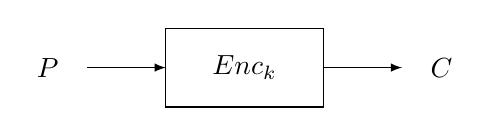
\begin{tikzpicture}
	  \draw[->,>=latex](-1, 0) -- (0, 0);	  
	  \draw[->,>=latex](2, 0) -- (3, 0);
	  \draw(-0, -.5) rectangle (2, .5);
	  \draw(1, 0) node {$Enc_{k}$};
	  \draw(-1.5, 0) node {$P$};
	  \draw(3.5, 0) node {$C$};
	\end{tikzpicture}
  \end{center}

  \begin{center}
	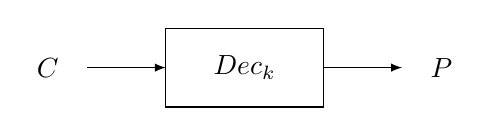
\begin{tikzpicture}
	  \draw[->,>=latex](-1, 0) -- (0, 0);	  
	  \draw[->,>=latex](2, 0) -- (3, 0);
	  \draw(-0, -.5) rectangle (2, .5);
	  \draw(1, 0) node {$Dec_{k}$};
	  \draw(-1.5, 0) node {$C$};
	  \draw(3.5, 0) node {$P$};
	\end{tikzpicture}
  \end{center}

  Where:
  $$
	P = 
	\begin{bmatrix}
	  x_{0} \\
	  x_{1} \\
	  \dots \\
	  x_{n}
	\end{bmatrix}
	\qquad
	C = 
	\begin{bmatrix}
	  y_{0} \\
	  y_{1} \\
	  \dots \\
	  y_{n}
	\end{bmatrix}
  $$

  Notice that the plaintext block and ciphertext block have the same
  length.

  \subsection{Rounds}

  A block algorithm is based on the repetition of short sequences of
  operations called \emph{rounds}.
  A round is a basic transformation which operates on a block. For
  example, an encryption algorithm could consist of three rounds: $C =
  R_{3} (R_{2}(R_{1}(P)))$. Each round should also have an
  \emph{inverse} in order to compute back the plaintext from the
  ciphertext: $P = R_{1}^{-1} (R_{2}^{-1}(R_{3}^{-1}(C)))$.
  
  There are two main techniques to build rounds:
  \emph{substitution-permutation networks} and \emph{Feistel
  schemes}.


  \subsubsection{Round keys and key schedule algorithm}

  Usually round functions ($R_{1},\dots R_{n}$) are the same, but they
  are parametrized by a \emph{round key}.
  A round key is a key which derives from the main key $K$.
  The same round function with different round keys will behave
  differently, and therefore will produce a different output blocks.

  An algorithm called \emph{key schedule} produces the round keys
  starting from the main key $K$.
  Round keys should always be different from each other in every round.
  

  \subsubsection{Substitution-permutation networks}  

  Substitution-permutation networks put together two important
  properties of cryptography\footnote{The terms \emph{confusion} and
  \emph{diffusion} were introduced by Claude Shannon.}:

  \begin{description}
	\item[Confusion:] the input (plaintext and key) undergoes
	  complex transformations, which make the relationship between the
	  statistics of the ciphertext and the value of the encryption key
	  as complex as possible. 
	\item[Diffusion:] the transformations depend equally on all bits
	  of the input, i.e. the ciphertext doesn't reflect the
	  statistical properties of the plaintext.
  \end{description}

  In a block cipher, a simple diffusion element is the bit
  \emph{permutation} (which is used frequently in DES),
  while confusion is achieved
  by the use of \emph{substitution} (used both in DES and in AES).

  \paragraph{Substitution:}
  
  Substitution boxes (S-boxes) 
  are small lookup tables that transform chunks of
  4 or 8 bits. For example, the 4-bit nibble $0000$ could be mapped to
  $0011$, while $0101$ could be mapped to $0110$, and so on.
  These S-boxes must be cryptographically strong (i.e. they
  should be as nonlinear as possible and have no statistical bias).

  \paragraph{Permutation:}
  The permutation could simply constist of a permutation of the bits,
  which is easy to implement but doesn't create to much diffusion.
  In practice different ciphers use operations from the linear algebra 
  to mix up the bits, like matrix-multiplications, and so on.
  Those operations create strong dependencies with all the bits of the
  input, and therefore ensure strong diffusion.

  \subsubsection{Feistel schemes}

  A Feistel scheme works as follows.:  
  \begin{enumerate}
	\item The input block is splitted in two halves, $L$ and $R$
	\item $L$ is XOR-ed with $F(R)$, where $F$ is a
	  substitution-permutation round
	\item $L$ and $R$ are swapped
	\item Step 2. and 3. are repeated a bunch of times
	\item $L$ and $R$ are merged into the output block
  \end{enumerate}

  \begin{center}
	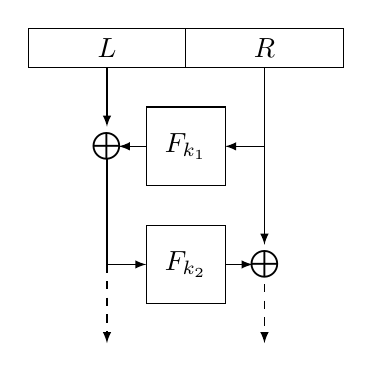
\begin{tikzpicture}
	  \draw(0, 3) rectangle (2, 3.5); 	  
	  \draw(1, 3.25) node {$L$};
	  \draw(2, 3) rectangle (4, 3.5);
	  \draw(3, 3.25) node {$R$};
	  \draw[->,>=latex](1, 3) -- (1, 2.25); %left arrow
	  \draw(1, 2) node {$\bigoplus$};
	  % arrow from R to F
	  \draw[->,>=latex](3, 3) -- (3, 2) -- (2.5, 2);
	  % F block
	  \draw(1.5, 1.5) rectangle (2.5, 2.5);
	  \draw(2, 2) node {$F_{k_{1}}$};
	  % arrow from F to XOR
	  \draw[->,>=latex](1.5, 2) -- (1.15, 2);
	  % arrow from XOR to F2
	  \draw(1.5, 0) rectangle (2.5, 1);
	  % XOR 2
	  \draw(3, .5) node {$\bigoplus$};
	  \draw[->,>=latex](3, 2) -- (3, .75);
	  \draw[->,>=latex](1, 1.85) -- (1, .5) -- (1.5, .5);
	  \draw(2, .5) node {$F_{k_{2}}$};
	  \draw[->,>=latex](2.5, .5) -- (2.85, .5);
	  \draw[->,>=latex,dashed](1, .5) -- (1, -.5);
	  \draw[->,>=latex,dashed](3, .25) -- (3, -.5);
	\end{tikzpicture}
  \end{center}

  Notice that $F_{k_{1}}$ and $F_{k_{2}}$ are actually the same
  function, they just take as input different round keys $K_{1}$ and
  $K_{2}$, which come from the key scheduling algorithm.
  

  \subsection{4$\times$4 S-box cipher}

  Howard M. Heys introduced this simple substitution-permutation based block 
  cipher in his lectures \emph{A Tutorial on Linear and Differential Algebra}.

  \paragraph{Substitution}
  \begin{itemize}
	\item The algorithm operates on 16-bit blocks.
	\item Each block is broken into four 4-bit sub-blocks.
	\item Each sub-block is fed into a $4\times4$ S-box (a
	  substitution-box with 4 input bits and 4 output bits). 
	\item In this case we use the same mapping for all
	  S-boxes\footnote{In DES all the S-boxes in a round are
	  different.}
	\item The S-box performs a \emph{nonlinear} mapping, i.e. the
	  output bits cannot be represented as a linear function of the
	  input bits.
  \end{itemize}

  The S-box used is the following:
  \begin{center}
	\begin{tabular}{|c|c|c|c|c|c|c|c|c|c|c|c|c|c|c|c|c|}
	  \hline
	  input & 0 & 1 & 2 & 3 & 4 & 5 & 6 & 7 & 8 & 9 & A & B & C & D & E & F \\
	  \hline
	  output & E & 4 & D & 1 & 2 & F & B & 8 & 3 & A & 6 & C & 5 & 9 &
	  0 & 7 \\
	  \hline
	\end{tabular}
  \end{center}

  You can verify that the mapping is nonlinear\footnote{A linear
  function maps a certain value $x$ into $k x$, where
  $k \in \mathbb{R}^{n}$} by simply observing
  that the number 0 is mapped to the hexadecimal value E 
  (which is 14 in decimal), while a linear function always maps the
  null-element 0 into 0 itself.
  Also, the mapping is not \emph{affine}:\footnote{An affine function
  maps a certain element $x$ into $kx+c$ where $k, c \in
  \mathbb{R}^{n}$.} while $\textrm{E}_{hex}$ = $14_{dec}$ = 0 + 14,
  instead $4 \neq 1 + 14$.

  \paragraph{Permutation}
  
  The permutation consists of a simple transposition of the bits, or
  the permutation of the bit positions.
  In the following \emph{permutation table} we represent for each
  input bit the position that it will take in the output (for example,
  the bit 2 is moved to position 5). 
  We stick with the author convention, in which $1$ is the
  rightmost bit and $16$ is the leftmost bit.
  \begin{center}
	\begin{tabular}{|c|c|c|c|c|c|c|c|c|c|c|c|c|c|c|c|c|}
	  \hline
	  input & 1 & 2 & 3 & 4 & 5 & 6 & 7 & 8 & 9 & 10 & 11 & 12 & 13 & 14 & 15& 16 \\
	  \hline
	  output & 1 & 5 & 9 & 13 & 2 & 6 & 10 & 14 & 3 & 7 & 11 & 15 & 4 & 8 &
	  12 & 16 \\
	  \hline
	\end{tabular}
  \end{center}
  
  \paragraph{Key mixing}

  To achieve key mixing, data blocks are XOR-ed with a round key
  before being fed into a S-box.


  % There are two main techniques to build a round:
  % \emph{substitution-permutation networks} and \emph{Feistel schemes}.
  
  \section{DES}
  
  \subsection{History} 

  In 1972 the US National Bureau of Standards (NBS, currently NIST)
  initiated a request for proposal for a standardized cipher in the
  USA. Up to this point in time cryptography had always been kept
  secret. By the early 70s, however, cryptography had become of
  crucial importance for a variety of commercial applications such as
  banking.

  The winning proposal selected in 1974 came from a team of
  cryptographers working at IBM.
  They submitted an algorithm based on the family of Feistel's ciphers 
  called \emph{Lucifer}, developed in the late 60s.

  In 1977 the NBS finally released all specifications of the IBM cipher 
  (which meanwhile had passed through some modifications) as 
  \emph{Data Encryption Standard} to the public. 
  However, the motivation for parts of the DES design\footnote{i.e.
  the design criteria.} were never officially released.
  During the following years, with the increase of personal computers
  in the early 80s, it became easier to analyze the inner structure of
  the cipher. However, no serious weaknesses were found until 1990.

  In 1999 DES was replaced by AES.

  \subsection{Description}

  DES is a symmetric block cipher which encrypts 64-bit blocks with a
  56-bit key. 

  \begin{center}
	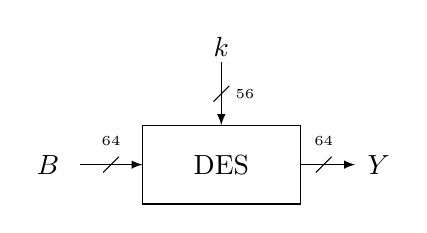
\begin{tikzpicture}
	  \draw(0, 0) rectangle (2,1);
	  \draw(1, 2) node {$k$};
	  \draw[->,>=latex](1, 1.8) -- (1, 1);
	  \draw(.9, 1.3) -- (1.1, 1.5);
	  \draw(1.3, 1.4) node {\tiny{56}};
	  \draw(1, .5) node {DES};
	  \draw[->,>=latex](-.8, .5) -- (0, .5);
	  \draw(-.5, .4) -- (-.3, .6);
	  \draw(-1.2, .5) node {$B$};
	  \draw(-.4, .8) node {\tiny{64}};
	  \draw[->,>=latex](2, .5) -- (2.7, .5);
	  \draw(2.2, .4) -- (2.4, .6);
	  \draw(2.3, .8) node {\tiny{64}};
	  \draw(3, .5) node {$Y$};
	\end{tikzpicture}
  \end{center}


  Each block passes through an initial bitwise permutation $IP$, then 
  16 rounds which all perform the identical operation, and eventually 
  a final bitwise permutation $IP^{-1}$, which is the inverse of the
  initial permutation $IP$.
  
  \begin{center}
	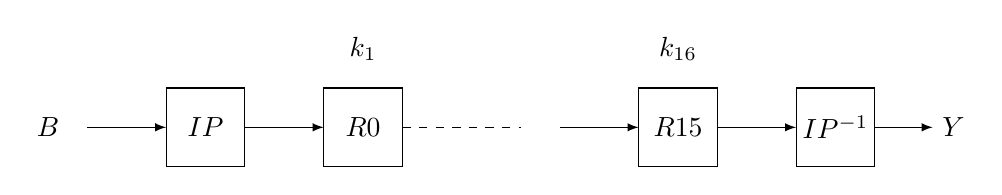
\begin{tikzpicture}
	  \draw(-1.5, .5) node(x) {$B$};  
	  \foreach \i / \txt in {0/$IP$,1/$R0$,3/$R15$,4/$IP^{-1}$}
	  {
		\draw(\i*2, 0) rectangle (\i*2+1, 1);
		\draw[->,>=latex](2*\i-1, .5) -- (2*\i, .5);
		\draw(\i*2+.5, .5) node {\txt};
	  }
	  \draw(2.5, 1.5) node {$k_{1}$};
	  \draw(6.5, 1.5) node {$k_{16}$};
	  \draw[dashed](3, .5) -- (4.5, .5);
	  \draw(10, .5) node(y) {$Y$};
	  \draw[->,>=latex](9, .5) -- (y);
	\end{tikzpicture}
  \end{center}

  In each round a different round key $k_{i}$ derived from the main
  key $k$ (with a key schedule) is used.
  Each DES round implements a Feistel scheme.
  
  \subsubsection{Internal permutation}

  The internal permutation $IP$ maps each input bit to an output bit.
  This doesn't increase security, it's just to arrange the plaintext. 
  The final permutation $IP^{-1}$ performs the reverse mapping.
  The following tables show the final position of each bit from $0$ to 63.
  The \hyperlink{appendix}{appendix} shows both the $IP$ and the
  $IP^{-1}$ structure.

  \subsubsection{The $f$ function}

  The Feistel function $f$ plays a crucial role for the security 
  of the DES cipher. In round $i$ it takes the right half 
  $R_{i-1}$ (32-bits) of the 
  output of the previous step and the round key $k_{i}$.
  The output is then XOR-ed with the left half of the previous step
  $L_{i-1}$ (32-bits).
  
  \begin{itemize}
	\item First, the 32-bit input is expanded to 48-bits by
	  partitioning the input into eight 4-bit blocks which are
	  expandend to 6-bit blocks with a $E$-box (a special type of
	  permutation). You can find the $E$-box in the
	  \hyperlink{appendix}{appendix}.

  
  \item Then the 48-bit result of the expansion is XOR-ed with the
	round key $k_{i}$, and the eight 6-bit blocks are fed into eight
	different S-boxes; each S-box maps a 6-bit block to a 4-bit
	block\footnote{Eight 4$\times$6 tables were close to the
	maximum size which could be fit on a single integrated circuit in
	1974.}.
	Each S-box contains $2^{6} = 64$ entries. Each entry is a 4-bit
	  value. The \hyperlink{appendix}{appendix} shows all the S-boxes.

	  The \emph{design criteria} behind the S-boxes are the following:
	  \begin{enumerate}
		\item Each S-box has 6 input bits and 4 output bits.
		\item No output bit of an S-box should be too close to a linear
		  combination of the input bits.
		\item If the lowest and highest bits of the input are fixed
		  and the four middle bits are varied, each of the possible
		  4-bit output values must occur exactly once.
		\item If two input to an S-box differ in exactly one bit,
		  their outputs must differ in at least two bits.
		\item If two inputs to an S-box differ in the two middle bits,
		  their outputs must differ in at least two bits.
		\item If two inputs to an S-box differ in their first two bits
		  and are identical in their last two bits, the two outputs
		  must be different.
		\item For any nonzero 6-bit difference between inputs, no more
		  than 8 of the 32 pairs of inputs exhibiting that difference
		  may result in the same output difference.
		\item A collision (zero output difference) at the 32-bit
		  output of the eight S-boxes is only possible for three
		  adjacent S-boxes.
	  \end{enumerate}

	  See \hyperlink{ex427}{Exercise 4.2.7} in which properties 3, 4,
	  5, 6 are checked.

	\item Finally, the 32-bit output passes through the $P$
	  permutation (see the \hyperlink{appendix}{appendix}).
	  This permutation introduces diffusion, because the four output
	  bits of each S-box are permuted in such a way that they affect
	  several different S-boxes in the following round.

	  The diffusion created by expansion, S-boxes and the $P$
	  permutation guarantees that each bit at the end of the fifth
	  round is a function of every plaintext bit and every key bit
	  (\emph{avalanche effect}).

  \end{itemize}

  The following picture represents the internal structure of the $f$
  function:

  \begin{center}
	\begin{tikzpicture}
	  \draw(-1.25, .25) node(r) {$R_{j}$};
	  \draw(0, 0) rectangle (1, .5) node[pos=.5] {$E$};
	  \draw[->,>=latex](-1, .25) -- (0, .25) node[midway, above]
	  {\tiny{32}} node[midway] {\tiny{/}};
	  \draw[->,>=latex](1, .25) -- (2, .25) node[midway,above]
	  {\tiny{48}} node[midway]{\tiny{/}};
	  \draw(2.2, .25) node {$\bigoplus$};
	  \draw(2.4, .25) -- (3, .25);
	  \draw[->,>=latex](2.2, 1) -- (2.2, .5);
	  \draw(2.2, 1.25) node(name) {$k_{j+1}$};
	  \draw(3, 3.75) -- (3, -3.25);
	  \foreach \i in {1,...,8}
	  {
		\draw[->,>=latex](3, 4.75-\i) -- +(1, 0) node[midway]
		{\tiny{/}} node[midway, above] {\tiny{6}};
		\draw(5, 4.75-\i) -- +(1, 0) node[midway] {\tiny{/}}
		node[midway,above] {\tiny{4}};
		\draw(4, 4.5-\i) rectangle +(1,.5) node[midway] {$S_{\i}$};
	  }
	  \draw(6, 3.75) -- (6, -3.25);
	  \draw[->,>=latex](6, .25) -- +(.5, 0);
	  \draw(6.5, 0) rectangle +(1, .5) node[midway] {$P$};
	  \draw[->,>=latex](7.5, .25) -- +(1, 0) node[midway]{\tiny{/}}
	  node[midway,above] {\tiny{32}};
	\end{tikzpicture}
  \end{center}

  See \hyperlink{ex4211}{Exercise 4.2.11} for an example of
  computation with the $f$ function.

  \subsubsection{The importance of being nonlinear}

  The S-boxes are at the core of DES in terms of cryptographic
  strength, because they produce confusion and are the \emph{only} 
  nonlinear element in the algorithm, i.e.:
  $$
	S(a) \oplus S(b) \neq S(a \oplus b)
  $$

  Why is nonlinearity so crucial? With a nonlinear building block, an
  attacker could express the DES input and output with a system of
  linear equations where the key bits are the unknowns. Such systems
  can easily be solved. S-boxes were carefully designed to
  prevent advanced mathematical attacks, such as \emph{differential
  cryptanalysis}.
  
  See \hyperlink{ex428}{Exercise 4.2.8} and \hyperlink{ex429}{Exercise
  4.2.9}.
  
  \subsection{Key schedule}

  The key schedule derives 16 round keys of from the main key $k$,
  each one consisting of 48-bits. 

  First, note that the DES input key is often stated as 64-bit, but
  every 7 bits there's an odd parity bit for the previous 7 bits.
  It's not clear why DES was specified that way, however the eight
  parity bits are not part of the actual key, they do not improve
  security, and therefore DES is a
  56-bit key cipher, not a 64-bit one.

  \begin{itemize}
	\item The parity bit are first removed from the key. Then the remaining
	  bits go through a permutation $PC-1$ (where $PC-1$ stands for
	  \emph{permuted choice one}). This permutation is shown in the
	  \hyperlink{appendix}{appendix}.
	\item The result is split into two halves $C_{0}$ and $D_{0}$.
	  The two 28-bit halves are cyclically shifted according to the
	  following rules:
	  \begin{itemize}
		\item In rounds $i = 1,2,9,16$ the two halves are rotated left
		  by one bit.
		\item In the other rounds, the two halves are rotated left by
		  two bits.
	  \end{itemize}
	\item To generate the 48-bit round keys $k_{i}$, the two halves
	  are permuted again with $PC-2$ (\emph{permuted choice 2}, see
	  \hyperlink{appendix}{appendix}), which
	  ignores the following bits: \texttt{9, 18, 22, 25, 35, 38, 43, 54}.
  \end{itemize}

  \subsection{Decryption}

  One advantage of DES is that decryption is the same function as
  encryption. This is because DES is based on a Feistel network.
  The only difference is the key schedule: the round keys are provided
  in reverse order (i.e. in round 1 round key 16 is needed, in round 2
  key 15, and so on).

  Because the total nubmber of rotations in the key schedule algorithm
  is 28, we have an interesting property: $C_{0} = C_{16}$ and $D_{0}
  = D_{16}$.
  Therefore, $k_{16}$ can be directly derived after
  $PC-1$\footnote{From now, we will omit the ‘-’ for clarity reasons.}:
  $$
	k_{16} = PC2(C_{16},D_{16}) = PC2(C_{0}, D_{0}) = PC2(PC1(k))	
  $$

  $k_{15}$ can be derived from $C_{16}, D_{16}$ through cyclic right
  shifts ($RS_{i}$):
  $$
	k_{15} = PC2(C_{15}, D_{15}) = PC2(RS_{2}(C_{16}),~
	RS_{2}(D_{16})) =
	PC2(RS_{2}(C_{0}), RS_{2}(D_{0}))
  $$

  \begin{itemize}
	\item In round 1 the key is not rotated.
	\item In rounds 2, 9 and 16 the two halves are rotated right by
	  one bit.
	\item In the other rounds the two halves are rotated right by two
	  bits.
  \end{itemize}
  
  \subsection{DES security}

  Ciphers can be attacked in several ways. With respect to
  cryptographic attacks, we distinguish between \emph{exhaustive key
  search} (or \emph{brute-force attacks}) and \emph{analytical
  attacks}.

  Although current analytical attacks against DES are not very
  efficient, DES can relatively easily be broken with an exhaustive
  key-search attack.
  This means that plain DES is not to be considered secure anymore.

  RSA security proposed several challenges to break DES, in order to
  prove that a 56-bit key is too short. During DES challenge III (1999),
  the EFF\footnote{Electronic Frontier Foundation.} decrypted a
  DES-encrypted message in 22 hours and 15 minutes by using Deep Crack, a 
  custom specifically built microchip.

  \subsubsection{3DES}

  A much stronger version of DES is 3DES, which consists of three
  subsequent DES encryptions with keys $k_{1}$, $k_{2}$, $k_{3}$.
  Usually 3DES is also implemented as EDE, i.e. the message is first
  encrypted with $k_{1}$, then decrypted with $k_{2}$ and finally
  encrypted with $k_{3}$.

  3DES seems resistant to both brute-force attacks and any known
  analytical attack.

  \subsubsection{2DES and meet-in-the-middle attack}
  
  We saw that 3DES is considered enough secure, but one could ask “Why
  not 2DES?”.
  The reason is quite simple: every block encryption algorithm, if
  applied two times, is vulnerable to the
  \emph{meet-in-the-middle-attack}.

  Let's consider a keylength of $\kappa$. Suppose that we first
  encrypt a plaintext by using a key $k_{1}$ and then we encrypt the
  ciphertext by using a key $k_{2}$.

  \begin{center}
	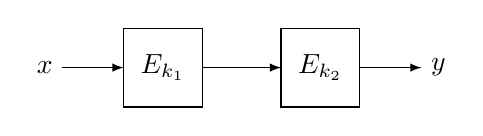
\begin{tikzpicture}
	  \draw(0, 0) node(x) {$x$};
	  \draw[->,>=latex](x) -- (1, 0);
	  \draw(1, -.5) rectangle (2, .5);
	  \draw(1.5, 0) node {$E_{k_{1}}$};
	  \draw[->,>=latex](2, 0) -- (3, 0);
	  \draw(3, -.5) rectangle (4, .5);
	  \draw(3.5, 0) node {$E_{k_{2}}$};
	  \draw(5, 0) node(y) {$y$};
	  \draw[->,>=latex](4, 0) -- (y);
	\end{tikzpicture}
  \end{center}

  A plain brute-force attack would require us to search through all
  possible combination of both keys, i.e. the effective key length
  would be $2\kappa$, and an exhaustive search would require
  $2^{\kappa} \cdot 2^{\kappa} = 2^{2\kappa}$ encryptions. 

  The meet-in-the-middle attack requires much more computational
  power:
  \begin{itemize}
	\item We (the adversary) know both the plaintext $x$ and the
	  ciphertext $y$.
	\item We first compute $2^{\kappa}$ encryptions of the
	  plaintext $x$, one  for each possible value of the key. 
	  We build a lookup table with all the encrypted values, indexed
	  by the value of $k_{1}$ that we used. 
	  In the case of DES, this would consist in $2^{56}$ operations.
	\item Then we start decrypting the ciphertext $y$ with all possible
	  values of the key $k_{2}$ ($2^{\kappa}$). 
	  If we find a match inside the lookup
	  table, then we have the key $k_{2}$. Not only: remember that the
	  lookup table is indexed by the value of $k_{1}$, this means that
	  we also have $k_{1}$. 
  \end{itemize}

  In the end, in the worst case we perform $2^{\kappa} + 2^{\kappa} =
  2\cdot 2^{\kappa} = 2^{\kappa + 1}$ operations, which are definitely
  less than $2^{2 \kappa}$.
  That's why double-encryption should be avoided with all the block
  ciphers.

  \paragraph{Example:}

  Let's say we have a plaintext $p$ and a ciphertext
  $c$.
  First we must encrypt $p$ with all possible $2^{\kappa}$ values of
  the key\footnote{For the sake of simplicity we consider just the
  decimal values.}:
  \begin{center}
	\begin{tabular}{|c|c|}
	  \hline
	  \texttt{k} & $\mathtt{Enc_{k}(p)}$ \\
	  \hline
	  \texttt{0} & \texttt{31269} \\
	  \hline
	  \texttt{1} & \texttt{161804} \\
	  \hline  
	  \dots & \dots \\
	  \hline
	  \dots & \dots \\
	  \hline
	  \texttt{$\mathtt{2^{\kappa-2}}$} & \texttt{21838121} \\
	  \hline
	  \texttt{$\mathtt{2^{\kappa-1}}$} & \texttt{193490} \\
	  \hline
	\end{tabular}
  \end{center}
  
  Then we start decrypting $c$ with all the possible $k_{2}$ key values.
  $$
	\mathtt{k=0} \Rightarrow \mathtt{Dec_{k}(c) = 1235443} 
  $$
  $$
	\mathtt{k=1} \Rightarrow \mathtt{Dec_{k}(c) = 21838121}
  $$

  We're lucky! It took us just two additional decryption to find a
  match. We look in the table and we see that the value
  \texttt{21838121} is in position $2^{\kappa-2}$. 
  In the end, the key $k_{1}$ is equal to $2^{\kappa-2}$, while the key $k_{2}$ is
  equal to 1, and we performed just $2^{\kappa} + 2$ computations.


  \section{Exercises}

  \hypertarget{ex427}{\paragraph{Exercise 4.2.7}}

  Check properties 3, 4, 5, 6 for S-box $S_{1}$.

  \begin{itemize}
	\item (3) It's easy to check that each row contains different
	  numbers. This means that for a fixed pair (first bit - last bit)
	  there are not two different middle bits configurations that produce the
	  same output.
	\item (4) Let's consider all the inputs which differ in exactly
	  one bit; you can check that the corresponding output bits will
	  differ in at least two bits. Let's take as an example the two
	  inputs 000000, which is mapped to 
	  $14 = 1110_{2}$, and 000001, which is mapped
	  to $0 = 0000_{2}$. While 000000 and
	  000001 differ in one bit, 1110 and
	  0000 differ in three bits.
	\item (5) Take as an example 000000, which is mapped to
	  $14 = 1110_{2}$ and 001100, which is mapped to 
	  $11 = 1011_{2}$. As you can see 1110 and
	  1011 differ in two bits.
	\item (6) Take as an example 000000, which is mapped to
	  $14 = 1110_{2}$ and 110000, which is mapped to
	$15 = 1111_{2}$. The output is clearly different.
  \end{itemize}

  \hypertarget{ex428}{\paragraph{Exercise 4.2.8}}

  Check that $S_{1}(4) \oplus S_{1}(23) \neq S_{1} (4 \oplus 23)$.

	  $$
		4 = 000100_{2}
		\qquad
		23 = 010111_{2}
	  $$
	  $$
		S_{1}(4) = 13 = 1101_{2}
		\qquad
		S_{1}(23) = 15 = 1111_{2}
	  $$
	  $$
		S_{1}(4 \oplus 23) = S_{1}(010011) = 6 = 0110_{2}
	  $$
	  $$
		S_{1}(4) \oplus S_{1}(23) = 0010_{2} = 2
	  $$
	  $$
		2 \neq 6
	  $$

	\hypertarget{ex429}{\paragraph{Exercise 4.2.9}}

	Check $S_{1}(0) \neq 0$. This shows that $S_{1}$ is non linear.
	$$
	  S_{1}(0) = 14 \neq 0
	$$

  \hypertarget{ex4211}{\paragraph{Exercise 4.2.11}}

  Compare the output of $f$ for inputs $R_{j} = 0$ and $R'_{j} = 1$
  with $k_{j+1} = 0$.

  \begin{itemize}
	\item First we compute the expansion through the $E$-box of both
	  $R_{j}$ and $R'_{j}$:
	  $$
		E(R_{j}) = 000\dots000 = 0^{48} 
		\qquad 
		E(R'_{j}) = 111\dots111 = 1^{48}
	  $$

	\item Then the expanded blocks are XOR-ed with the key $k_{j+1} =
	  0^{48}$:
	  $$
		E(R_{j})\oplus k_{j+1} = 0^{48}
		\qquad
		E(R'_{j})\oplus k_{j+1} = 1^{48}
	  $$

	\item Now we divide the 48-bit blocks in eight 6-bit sub blocks,
	  which are sent to the S-boxes. In this the sub blocks $B_{j}$ are all
	  the same:
	  $$
		B_{j} = 0^{6}
		\qquad
		B'_{j} = 1^{6}
	  $$
	  Let's apply the S-boxes to each block:
	  \begin{center}
		\begin{tabular}{crr}
		  $S_{1}(B_{j}) = $ & $14 = $ & $1110$ \\
		  $S_{2}(B_{j}) = $ & $15 = $ & $1111$ \\
		  $S_{3}(B_{j}) = $ & $10 = $ & $1010$ \\
		  $S_{4}(B_{j}) = $ & $7  = $ & $0111$ \\
		  $S_{5}(B_{j}) = $ & $2  = $ & $0010$ \\
		  $S_{6}(B_{j}) = $ & $12 = $ & $1100$ \\
		  $S_{7}(B_{j}) = $ & $4  = $ & $0100$ \\
		  $S_{8}(B_{j}) = $ & $13 = $ & $1101$ \\
		\end{tabular}
		\qquad
		\begin{tabular}{crr}
		  $S_{1}(B'_{j}) = $ & $13 = $ & $1101$ \\
		  $S_{2}(B'_{j}) = $ & $9  = $ & $0101$ \\
		  $S_{3}(B'_{j}) = $ & $12 = $ & $1100$ \\
		  $S_{4}(B'_{j}) = $ & $14 = $ & $1110$ \\
		  $S_{5}(B'_{j}) = $ & $3  = $ & $0011$ \\
		  $S_{6}(B'_{j}) = $ & $13 = $ & $1101$ \\
		  $S_{7}(B'_{j}) = $ & $12 = $ & $1100$ \\
		  $S_{8}(B'_{j}) = $ & $11 = $ & $1011$ \\
		\end{tabular}
	  \end{center}

	\item Finally, we apply $P$ to the concatenation of all the bits:
	  $$
		P(11101111101001110010110001001101) = 
	  $$
	  $$
		= f(R_{j}) =  11011000110110001101101110111100
	  $$
	  $$
		P(11010101110011100011110111001011) =
		$$
	  $$
		= f(R'_{j}) = 00111000110100111111100111011011
	  $$

  \end{itemize}



  \appendix
  \hypertarget{appendix}{\section{Appendix}}

  Read from left to right, top to bottom.

  \begin{center}
	$IP$ \\
	\vspace{10pt}
	\begin{tabular}{|cccccccc|}
	  \hline
	  \texttt{58} & \texttt{50} & \texttt{42} & \texttt{34} & \texttt{26} & \texttt{18} & \texttt{10} & \texttt{2} \\
	  \hline
	  \texttt{60} & \texttt{52} & \texttt{44} & \texttt{36} & \texttt{28} & \texttt{20} & \texttt{12} & \texttt{4} \\
	  \hline
	  \texttt{62} & \texttt{54} & \texttt{46} & \texttt{38} & \texttt{30} & \texttt{22} & \texttt{14} & \texttt{6} \\
	  \hline
	  \texttt{64} & \texttt{56} & \texttt{48} & \texttt{40} & \texttt{32} & \texttt{24} & \texttt{16} & \texttt{8} \\
	  \hline
	  \texttt{57} & \texttt{49} & \texttt{41} & \texttt{33} & \texttt{25} & \texttt{17} & \texttt{9} & \texttt{1} \\
	  \hline
	  \texttt{59} & \texttt{51} & \texttt{43} & \texttt{35} & \texttt{27} & \texttt{19} & \texttt{11} & \texttt{3} \\
	  \hline
	  \texttt{61} & \texttt{53} & \texttt{45} & \texttt{37} & \texttt{29} & \texttt{21} & \texttt{13} & \texttt{5} \\
	  \hline
	  \texttt{63} & \texttt{55} & \texttt{47} & \texttt{39} & \texttt{31} & \texttt{23} & \texttt{15} & \texttt{7} \\
	  \hline
	\end{tabular}
  \end{center}

  \begin{center}
	$IP^{-1}$ \\
	\vspace{10pt}
	\begin{tabular}{|cccccccc|}
	  \hline
\texttt{40} & \texttt{8} & \texttt{48} & \texttt{16} & \texttt{56} & \texttt{24} & \texttt{64} & \texttt{32} \\
	  \hline
\texttt{39} & \texttt{7} & \texttt{47} & \texttt{15} & \texttt{55} & \texttt{23} & \texttt{63} & \texttt{31} \\
	  \hline
\texttt{38} & \texttt{6} & \texttt{46} & \texttt{14} & \texttt{54} & \texttt{22} & \texttt{62} & \texttt{30} \\
	  \hline
\texttt{37} & \texttt{5} & \texttt{45} & \texttt{13} & \texttt{53} & \texttt{21} & \texttt{61} & \texttt{29} \\
	  \hline
\texttt{36} & \texttt{4} & \texttt{44} & \texttt{12} & \texttt{52} & \texttt{20} & \texttt{60} & \texttt{28} \\
	  \hline
\texttt{35} & \texttt{3} & \texttt{43} & \texttt{11} & \texttt{51} & \texttt{19} & \texttt{59} & \texttt{27} \\
	  \hline
\texttt{34} & \texttt{2} & \texttt{42} & \texttt{10} & \texttt{50} & \texttt{18} & \texttt{58} & \texttt{26} \\
	  \hline
\texttt{33} & \texttt{1} & \texttt{41} & \texttt{9} & \texttt{49} & \texttt{17} & \texttt{57} & \texttt{25}  \\
	  \hline
  \end{tabular}
  \end{center}

  \begin{center}
	$E$ \\
	\vspace{5pt}
	\begin{tabular}{|cccccc|}
	  \hline
	  \texttt{32} & \texttt{1} & \texttt{2} & \texttt{3} & \texttt{4} & \texttt{5} \\
	  \hline
	  \texttt{4} & \texttt{5} & \texttt{6} & \texttt{7} & \texttt{8} & \texttt{9} \\
	  \hline
	  \texttt{8} & \texttt{9} & \texttt{10} & \texttt{11} & \texttt{12} & \texttt{13} \\
	  \hline
	  \texttt{12} & \texttt{13} & \texttt{14} & \texttt{15} & \texttt{16} & \texttt{17} \\
	  \hline
	  \texttt{16} & \texttt{17} & \texttt{18} & \texttt{19} & \texttt{20} & \texttt{21} \\
	  \hline
	  \texttt{20} & \texttt{21} & \texttt{22} & \texttt{23} & \texttt{24} & \texttt{25} \\
	  \hline
	  \texttt{24} & \texttt{25} & \texttt{26} & \texttt{27} & \texttt{28} & \texttt{29} \\
	  \hline
	  \texttt{28} & \texttt{29} & \texttt{30} & \texttt{31} & \texttt{32} & \texttt{1} \\
	  \hline
	\end{tabular}
  \end{center}

  \vspace{20pt}

  \begin{center}
	\emph{S-boxes}
  \end{center}
	\textbf{How to read:} each row is indexed by the concatenation of the rightmost 
	and the leftmost bit of the 6-bit value, while each column is
	indexed by the 4 middle bits (represented in decimal for
	compactness reasons). For example if the input is \texttt{001101},
	the row is the one with label \texttt{01} (first and last bit) while 
	the column is the one with label \texttt{0110} = \texttt{6}.

  \begin{center}

\begin{tabular}{|c|cccccccccccccccc|}
  \hline
\texttt{S1} & \texttt{0} & \texttt{1} & \texttt{2} & \texttt{3} & \texttt{4} & \texttt{5} & \texttt{6} & \texttt{7} & \texttt{8} & \texttt{9} & \texttt{10} & \texttt{11} & \texttt{12} & \texttt{13} & \texttt{14} & \texttt{15} \\
\hline
\texttt{00} & \texttt{14} & \texttt{4} & \texttt{13} & \texttt{1} & \texttt{2} & \texttt{15} & \texttt{11} & \texttt{8} & \texttt{3} & \texttt{10} & \texttt{6} & \texttt{12} & \texttt{5} & \texttt{9} & \texttt{0} & \texttt{7} \\
\texttt{01} & \texttt{0} & \texttt{15} & \texttt{7} & \texttt{4} & \texttt{14} & \texttt{2} & \texttt{13} & \texttt{1} & \texttt{10} & \texttt{6} & \texttt{12} & \texttt{11} & \texttt{9} & \texttt{5} & \texttt{3} & \texttt{8} \\
\texttt{10} & \texttt{4} & \texttt{1} & \texttt{14} & \texttt{8} & \texttt{13} & \texttt{6} & \texttt{2} & \texttt{11} & \texttt{15} & \texttt{12} & \texttt{9} & \texttt{7} & \texttt{3} & \texttt{10} & \texttt{5} & \texttt{0} \\
\texttt{11} & \texttt{15} & \texttt{12} & \texttt{8} & \texttt{2} & \texttt{4} & \texttt{9} & \texttt{1} & \texttt{7} & \texttt{5} & \texttt{11} & \texttt{3} & \texttt{14} & \texttt{10} & \texttt{0} & \texttt{6} & \texttt{13} \\
  \hline
\end{tabular}

\vspace{10pt}
\begin{tabular}{|c|cccccccccccccccc|}
  \hline
\texttt{S2} & \texttt{0} & \texttt{1} & \texttt{2} & \texttt{3} & \texttt{4} & \texttt{5} & \texttt{6} & \texttt{7} & \texttt{8} & \texttt{9} & \texttt{10} & \texttt{11} & \texttt{12} & \texttt{13} & \texttt{14} & \texttt{15} \\
\hline
\texttt{00} & \texttt{1}\texttt{5} & \texttt{1} & \texttt{8} & \texttt{1}\texttt{4} & \texttt{6} & \texttt{1}\texttt{1} & \texttt{3} & \texttt{4} & \texttt{9} & \texttt{7} & \texttt{2} & \texttt{1}\texttt{3} & \texttt{1}\texttt{2} & \texttt{0} & \texttt{5} & \texttt{1}\texttt{0} \\
\texttt{01} & \texttt{3} & \texttt{1}\texttt{3} & \texttt{4} & \texttt{7} & \texttt{1}\texttt{5} & \texttt{2} & \texttt{8} & \texttt{1}\texttt{4} & \texttt{1}\texttt{2} & \texttt{0} & \texttt{1} & \texttt{1}\texttt{0} & \texttt{6} & \texttt{9} & \texttt{1}\texttt{1} & \texttt{5} \\
\texttt{10} & \texttt{0} & \texttt{1}\texttt{4} & \texttt{7} & \texttt{1}\texttt{1} & \texttt{1}\texttt{0} & \texttt{4} & \texttt{1}\texttt{3} & \texttt{1} & \texttt{5} & \texttt{8} & \texttt{1}\texttt{2} & \texttt{6} & \texttt{9} & \texttt{3} & \texttt{2} & \texttt{1}\texttt{5} \\
\texttt{11} & \texttt{1}\texttt{3} & \texttt{8} & \texttt{1}\texttt{0} & \texttt{1} & \texttt{3} & \texttt{1}\texttt{5} & \texttt{4} & \texttt{2} & \texttt{1}\texttt{1} & \texttt{6} & \texttt{7} & \texttt{1}\texttt{2} & \texttt{0} & \texttt{5} & \texttt{1}\texttt{4} & \texttt{9} \\
\hline
\end{tabular}

\vspace{10pt}
\begin{tabular}{|c|cccccccccccccccc|}
  \hline
\texttt{S3} & \texttt{0} & \texttt{1} & \texttt{2} & \texttt{3} & \texttt{4} & \texttt{5} & \texttt{6} & \texttt{7} & \texttt{8} & \texttt{9} & \texttt{10} & \texttt{11} & \texttt{12} & \texttt{13} & \texttt{14} & \texttt{15} \\
\hline
\texttt{0}\texttt{0} & \texttt{1}\texttt{0} & \texttt{0} & \texttt{9} & \texttt{1}\texttt{4} & \texttt{6} & \texttt{3} & \texttt{1}\texttt{5} & \texttt{5} & \texttt{1} & \texttt{1}\texttt{3} & \texttt{1}\texttt{2} & \texttt{7} & \texttt{1}\texttt{1} & \texttt{4} & \texttt{2} & \texttt{8} \\
\texttt{0}\texttt{1} & \texttt{1}\texttt{3} & \texttt{7} & \texttt{0} & \texttt{9} & \texttt{3} & \texttt{4} & \texttt{6} & \texttt{1}\texttt{0} & \texttt{2} & \texttt{8} & \texttt{5} & \texttt{1}\texttt{4} & \texttt{1}\texttt{2} & \texttt{1}\texttt{1} & \texttt{1}\texttt{5} & \texttt{1} \\
\texttt{1}\texttt{0} & \texttt{1}\texttt{3} & \texttt{6} & \texttt{4} & \texttt{9} & \texttt{8} & \texttt{1}\texttt{5} & \texttt{3} & \texttt{0} & \texttt{1}\texttt{1} & \texttt{1} & \texttt{2} & \texttt{1}\texttt{2} & \texttt{5} & \texttt{1}\texttt{0} & \texttt{1}\texttt{4} & \texttt{7} \\
\texttt{1}\texttt{1} & \texttt{1} & \texttt{1}\texttt{0} & \texttt{1}\texttt{3} & \texttt{0} & \texttt{6} & \texttt{9} & \texttt{8} & \texttt{7} & \texttt{4} & \texttt{1}\texttt{5} & \texttt{1}\texttt{4} & \texttt{3} & \texttt{1}\texttt{1} & \texttt{5} & \texttt{2} & \texttt{1}\texttt{2}  \\
\hline
\end{tabular}


\vspace{10pt}
\begin{tabular}{|c|cccccccccccccccc|}
  \hline
\texttt{S4} & \texttt{0} & \texttt{1} & \texttt{2} & \texttt{3} & \texttt{4} & \texttt{5} & \texttt{6} & \texttt{7} & \texttt{8} & \texttt{9} & \texttt{10} & \texttt{11} & \texttt{12} & \texttt{13} & \texttt{14} & \texttt{15} \\
\hline
\texttt{0}\texttt{0} & \texttt{7} & \texttt{1}\texttt{3} & \texttt{1}\texttt{4} & \texttt{3} & \texttt{0} & \texttt{6} & \texttt{9} & \texttt{1}\texttt{0} & \texttt{1} & \texttt{2} & \texttt{8} & \texttt{5} & \texttt{1}\texttt{1} & \texttt{1}\texttt{2} & \texttt{4} & \texttt{1}\texttt{5} \\
\texttt{0}\texttt{1} & \texttt{1}\texttt{3} & \texttt{8} & \texttt{1}\texttt{1} & \texttt{5} & \texttt{6} & \texttt{1}\texttt{5} & \texttt{0} & \texttt{3} & \texttt{4} & \texttt{7} & \texttt{2} & \texttt{1}\texttt{2} & \texttt{1} & \texttt{1}\texttt{0} & \texttt{1}\texttt{4} & \texttt{9} \\
\texttt{1}\texttt{0} & \texttt{1}\texttt{0} & \texttt{6} & \texttt{9} & \texttt{0} & \texttt{1}\texttt{2} & \texttt{1}\texttt{1} & \texttt{7} & \texttt{1}\texttt{3} & \texttt{1}\texttt{5} & \texttt{1} & \texttt{3} & \texttt{1}\texttt{4} & \texttt{5} & \texttt{2} & \texttt{8} & \texttt{4} \\
\texttt{1}\texttt{1} & \texttt{3} & \texttt{1}\texttt{5} & \texttt{0} & \texttt{6} & \texttt{1}\texttt{0} & \texttt{1} & \texttt{1}\texttt{3} & \texttt{8} & \texttt{9} & \texttt{4} & \texttt{5} & \texttt{1}\texttt{1} & \texttt{1}\texttt{2} & \texttt{7} & \texttt{2} & \texttt{1}\texttt{4} \\
\hline
\end{tabular}

\vspace{10pt}
\begin{tabular}{|c|cccccccccccccccc|}
  \hline
\texttt{S5} & \texttt{0} & \texttt{1} & \texttt{2} & \texttt{3} & \texttt{4} & \texttt{5} & \texttt{6} & \texttt{7} & \texttt{8} & \texttt{9} & \texttt{10} & \texttt{11} & \texttt{12} & \texttt{13} & \texttt{14} & \texttt{15} \\
\hline
\texttt{0}\texttt{0} & \texttt{2} & \texttt{1}\texttt{2} & \texttt{4} & \texttt{1} & \texttt{7} & \texttt{1}\texttt{0} & \texttt{1}\texttt{1} & \texttt{6} & \texttt{8} & \texttt{5} & \texttt{3} & \texttt{1}\texttt{5} & \texttt{1}\texttt{3} & \texttt{0} & \texttt{1}\texttt{4} & \texttt{9} \\
\texttt{0}\texttt{1} & \texttt{1}\texttt{4} & \texttt{1}\texttt{1} & \texttt{2} & \texttt{1}\texttt{2} & \texttt{4} & \texttt{7} & \texttt{1}\texttt{3} & \texttt{1} & \texttt{5} & \texttt{0} & \texttt{1}\texttt{5} & \texttt{1}\texttt{0} & \texttt{3} & \texttt{9} & \texttt{8} & \texttt{6} \\
\texttt{1}\texttt{0} & \texttt{4} & \texttt{2} & \texttt{1} & \texttt{1}\texttt{1} & \texttt{1}\texttt{0} & \texttt{1}\texttt{3} & \texttt{7} & \texttt{8} & \texttt{1}\texttt{5} & \texttt{9} & \texttt{1}\texttt{2} & \texttt{5} & \texttt{6} & \texttt{3} & \texttt{0} & \texttt{1}\texttt{4} \\
\texttt{1}\texttt{1} & \texttt{1}\texttt{1} & \texttt{8} & \texttt{1}\texttt{2} & \texttt{7} & \texttt{1} & \texttt{1}\texttt{4} & \texttt{2} & \texttt{1}\texttt{3} & \texttt{6} & \texttt{1}\texttt{5} & \texttt{0} & \texttt{9} & \texttt{1}\texttt{0} & \texttt{4} & \texttt{5} & \texttt{3} \\
\hline
\end{tabular}

\vspace{10pt}
\begin{tabular}{|c|cccccccccccccccc|}
  \hline
\texttt{S6} & \texttt{0} & \texttt{1} & \texttt{2} & \texttt{3} & \texttt{4} & \texttt{5} & \texttt{6} & \texttt{7} & \texttt{8} & \texttt{9} & \texttt{10} & \texttt{11} & \texttt{12} & \texttt{13} & \texttt{14} & \texttt{15} \\
\hline
\texttt{0}\texttt{0} & \texttt{1}\texttt{2} & \texttt{1} & \texttt{1}\texttt{0} & \texttt{1}\texttt{5} & \texttt{9} & \texttt{2} & \texttt{6} & \texttt{8} & \texttt{0} & \texttt{1}\texttt{3} & \texttt{3} & \texttt{4} & \texttt{1}\texttt{4} & \texttt{7} & \texttt{5} & \texttt{1}\texttt{1} \\
\texttt{0}\texttt{1} & \texttt{1}\texttt{0} & \texttt{1}\texttt{5} & \texttt{4} & \texttt{2} & \texttt{7} & \texttt{1}\texttt{2} & \texttt{9} & \texttt{5} & \texttt{6} & \texttt{1} & \texttt{1}\texttt{3} & \texttt{1}\texttt{4} & \texttt{0} & \texttt{1}\texttt{1} & \texttt{3} & \texttt{8} \\
\texttt{1}\texttt{0} & \texttt{9} & \texttt{1}\texttt{4} & \texttt{1}\texttt{5} & \texttt{5} & \texttt{2} & \texttt{8} & \texttt{1}\texttt{2} & \texttt{3} & \texttt{7} & \texttt{0} & \texttt{4} & \texttt{1}\texttt{0} & \texttt{1} & \texttt{1}\texttt{3} & \texttt{1}\texttt{1} & \texttt{6} \\
\texttt{1}\texttt{1} & \texttt{4} & \texttt{3} & \texttt{2} & \texttt{1}\texttt{2} & \texttt{9} & \texttt{5} & \texttt{1}\texttt{5} & \texttt{1}\texttt{0} & \texttt{1}\texttt{1} & \texttt{1}\texttt{4} & \texttt{1} & \texttt{7} & \texttt{6} & \texttt{0} & \texttt{8} & \texttt{1}\texttt{3} \\
\hline
\end{tabular}

\vspace{10pt}
\begin{tabular}{|c|cccccccccccccccc|}
  \hline
\texttt{S7} & \texttt{0} & \texttt{1} & \texttt{2} & \texttt{3} & \texttt{4} & \texttt{5} & \texttt{6} & \texttt{7} & \texttt{8} & \texttt{9} & \texttt{10} & \texttt{11} & \texttt{12} & \texttt{13} & \texttt{14} & \texttt{15} \\
\hline
\texttt{0}\texttt{0} & \texttt{4} & \texttt{1}\texttt{1} & \texttt{2} & \texttt{1}\texttt{4} & \texttt{1}\texttt{5} & \texttt{0} & \texttt{8} & \texttt{1}\texttt{3} & \texttt{3} & \texttt{1}\texttt{2} & \texttt{9} & \texttt{7} & \texttt{5} & \texttt{1}\texttt{0} & \texttt{6} & \texttt{1} \\
\texttt{0}\texttt{1} & \texttt{1}\texttt{3} & \texttt{0} & \texttt{1}\texttt{1} & \texttt{7} & \texttt{4} & \texttt{9} & \texttt{1} & \texttt{1}\texttt{0} & \texttt{1}\texttt{4} & \texttt{3} & \texttt{5} & \texttt{1}\texttt{2} & \texttt{2} & \texttt{1}\texttt{5} & \texttt{8} & \texttt{6} \\
\texttt{1}\texttt{0} & \texttt{1} & \texttt{4} & \texttt{1}\texttt{1} & \texttt{1}\texttt{3} & \texttt{1}\texttt{2} & \texttt{3} & \texttt{7} & \texttt{1}\texttt{4} & \texttt{1}\texttt{0} & \texttt{1}\texttt{5} & \texttt{6} & \texttt{8} & \texttt{0} & \texttt{5} & \texttt{9} & \texttt{2} \\
\texttt{1}\texttt{1} & \texttt{6} & \texttt{1}\texttt{1} & \texttt{1}\texttt{3} & \texttt{8} & \texttt{1} & \texttt{4} & \texttt{1}\texttt{0} & \texttt{7} & \texttt{9} & \texttt{5} & \texttt{0} & \texttt{1}\texttt{5} & \texttt{1}\texttt{4} & \texttt{2} & \texttt{3} & \texttt{1}\texttt{2} \\
\hline
\end{tabular}

\vspace{10pt}
\begin{tabular}{|c|cccccccccccccccc|}
  \hline
\texttt{S8} & \texttt{0} & \texttt{1} & \texttt{2} & \texttt{3} & \texttt{4} & \texttt{5} & \texttt{6} & \texttt{7} & \texttt{8} & \texttt{9} & \texttt{10} & \texttt{11} & \texttt{12} & \texttt{13} & \texttt{14} & \texttt{15} \\
\hline
\texttt{0}\texttt{0} & \texttt{1}\texttt{3} & \texttt{2} & \texttt{8} & \texttt{4} & \texttt{6} & \texttt{1}\texttt{5} & \texttt{1}\texttt{1} & \texttt{1} & \texttt{1}\texttt{0} & \texttt{9} & \texttt{3} & \texttt{1}\texttt{4} & \texttt{5} & \texttt{0} & \texttt{1}\texttt{2} & \texttt{7} \\
\texttt{0}\texttt{1} & \texttt{1} & \texttt{1}\texttt{5} & \texttt{1}\texttt{3} & \texttt{8} & \texttt{1}\texttt{0} & \texttt{3} & \texttt{7} & \texttt{4} & \texttt{1}\texttt{2} & \texttt{5} & \texttt{6} & \texttt{1}\texttt{1} & \texttt{0} & \texttt{1}\texttt{4} & \texttt{9} & \texttt{2} \\
\texttt{1}\texttt{0} & \texttt{7} & \texttt{1}\texttt{1} & \texttt{4} & \texttt{1} & \texttt{9} & \texttt{1}\texttt{2} & \texttt{1}\texttt{4} & \texttt{2} & \texttt{0} & \texttt{6} & \texttt{1}\texttt{0} & \texttt{1}\texttt{3} & \texttt{1}\texttt{5} & \texttt{3} & \texttt{5} & \texttt{8} \\
\texttt{1}\texttt{1} & \texttt{2} & \texttt{1} & \texttt{1}\texttt{4} & \texttt{7} & \texttt{4} & \texttt{1}\texttt{0} & \texttt{8} & \texttt{1}\texttt{3} & \texttt{1}\texttt{5} & \texttt{1}\texttt{2} & \texttt{9} & \texttt{0} & \texttt{3} & \texttt{5} & \texttt{6} & \texttt{1}\texttt{1} \\
\hline
\end{tabular}

\vspace{20pt}

$P$ \\
\vspace{10pt}
\begin{tabular}{|cccccccc|}
\hline
\texttt{16} &  \texttt{7} &  \texttt{20} &  \texttt{21} &  \texttt{29} &  \texttt{12} &  \texttt{28} &  \texttt{17} \\
\hline
\texttt{1} &  \texttt{15} &  \texttt{23} &  \texttt{26} &  \texttt{5} &  \texttt{18} &  \texttt{31} &  \texttt{10} \\
\hline
\texttt{2} &  \texttt{8} &  \texttt{24} &  \texttt{14} &  \texttt{32} &  \texttt{27} &  \texttt{3} &  \texttt{9} \\
\hline
\texttt{19} &  \texttt{13} &  \texttt{30} &  \texttt{6} &  \texttt{22} &  \texttt{11} &  \texttt{4} &  \texttt{25} \\
\hline
\end{tabular}


\vspace{20pt}

$PC-1$ 
\vspace{10pt}

\begin{tabular}{|cccccccc|}
\hline
\texttt{57} & \texttt{49} & \texttt{41} & \texttt{33} & \texttt{25} & \texttt{17} & \texttt{9} & \texttt{1} \\
\hline
\texttt{58} & \texttt{50} & \texttt{42} & \texttt{34} & \texttt{26} & \texttt{18} & \texttt{10} & \texttt{2} \\
\hline
\texttt{59} & \texttt{51} & \texttt{43} & \texttt{35} & \texttt{27} & \texttt{19} & \texttt{11} & \texttt{3} \\
\hline
\texttt{60} & \texttt{52} & \texttt{44} & \texttt{36} & \texttt{63} & \texttt{55} & \texttt{47} & \texttt{39} \\
\hline
\texttt{31} & \texttt{23} & \texttt{15} & \texttt{7} & \texttt{62} & \texttt{54} & \texttt{46} & \texttt{38} \\
\hline
\texttt{30} & \texttt{22} & \texttt{14} & \texttt{6} & \texttt{61} & \texttt{53} & \texttt{45} & \texttt{37} \\
\hline
\texttt{29} & \texttt{21} & \texttt{13} & \texttt{5} & \texttt{28} & \texttt{20} & \texttt{12} & \texttt{4} \\
\hline
\end{tabular}

\vspace{20pt}

$PC-2$ \\
\vspace{10pt}
\begin{tabular}{|cccccccc|}
\hline
\texttt{14} & \texttt{17} & \texttt{11} & \texttt{24} & \texttt{1} & \texttt{5} & \texttt{3} & \texttt{28}\\
\hline
\texttt{15} & \texttt{6} & \texttt{21} & \texttt{10} & \texttt{23} & \texttt{19} & \texttt{12} & \texttt{4}\\
\hline
\texttt{26} & \texttt{8} & \texttt{16} & \texttt{7} & \texttt{27} & \texttt{20} & \texttt{13} & \texttt{2}\\
\hline
\texttt{41} & \texttt{52} & \texttt{31} & \texttt{37} & \texttt{47} & \texttt{55} & \texttt{30} & \texttt{40}\\
\hline
\texttt{51} & \texttt{45} & \texttt{33} & \texttt{48} & \texttt{44} & \texttt{49} & \texttt{39} & \texttt{56}\\
\hline
\texttt{34} & \texttt{53} & \texttt{46} & \texttt{42} & \texttt{50} & \texttt{36} & \texttt{29} & \texttt{32}\\
\hline
\end{tabular}

  \end{center}
  %%%%%%%%%%%%%%%%%%%%%%%%%%%%%%%%%%%%%%%%%%%%%%%%%%%%%%%%%%%%%%%%%%%%
  %LESSON 8: 25-03-2021%
 \section{AES: Introduction}
AES (aka Rijndael from its invetor's name) is a block ciphers  with blocks of 128 (27) bits. It is important that blocks are not too large in order to minimize both the length of ciphertext and the memory footprint.
As for the memory footprint, in order to process a 128-bit block, you need at least 128 bits of memory. This is small enough to fit in the registers of most CPUs or to be implemented using dedicated hardware circuits. Blocks of 64, 128, or even 512 bits are short enough to allow for efficient implementations in most cases.
When ciphertexts’ length or memory footprint is critical, you may have to use 64-bit blocks, because these will produce shorter ciphertexts and consume less memory. If it is possible , 128-bit or larger blocks are better. If you need to encrypt a 16-bit message when blocks are 128 bits, you’ll first need to convert the message into a 128-bit block by means of padding. Blocks shouldn’t be too small otherwise, they may be susceptible to codebook attacks. The codebook attack works like this with 16-bit blocks:
1. Get the 65536 (216) ciphertexts corresponding to each 16-bit
plaintext block.
2. Build a lookup table—the codebook—mapping each ciphertext block
to its corresponding plaintext block.
3. To decrypt an unknown ciphertext block, look up its corresponding
plaintext block in the table.
\section*{Rounds}
Computing a block cipher boils down to computing a sequence of rounds.
In a block cipher, a round is a basic transformation that is simple to specify and to implement, and which is iterated several times. Each round should also have an inverse in order to make it possible for a recipient to compute back to plaintext. The round functions—R1, R2, and so on—are usually identical algorithms, but they are parameterized by a value called the round key.
In a block cipher, no round should be identical to another round in order to avoid a slide attack. When rounds are identical, the relation between the two plaintexts, P2 = R(P1), implies the relation C2 = R(C1). Knowing the input and output of a single round often helps recover the key.
\begin{figure}[htb]
	\begin{center}
  		\includegraphics[width=0.75 \textwidth,]{rounds.png} 
 	\end{center}
\end{figure}

\newpage
\section{Confusion and DIffusion}
Confusion means that the input (plaintext and encryption key) undergoes complex transformations so that it is hard to recover the key having ciphertext (at a high level, confusion is about depth whereas diffusion is about breadth). 
Diffusion means that these transformations depend equally on all bits of the input (ability of distribute the statistical correlation among the entire alphabet used by the algorithm, making harder a statistical attack which means that some letters are more used than other and the same for the combination of letter) . 
In the design of a block cipher, confusion and diffusion take the form of substitution and permutation operations, which are combined within substitution–permutation networks (SPNs).
Substitution often appears in the form of S-boxes, or substitution boxes, which are small lookup tables that transform chunks of 4 or 8 bits (S-boxes should be as nonlinear as possible).
The permutation can be as simple as changing the order of the bits, which is easy to implement but does not mix up the bits very much. Some ciphers use basic linear algebra and matrix multiplications to mix up the bits: they perform a series of multiplication operations with fixed values (the matrix’s coefficients) and then add the results.
\section{AES}
AES processes blocks of 128 bits using a secret key of 128, 192, or 256 bits (the number of transformation rounds that convert the plaintext into the ciphertext depends on the length of the key). The 128-bit key being the most common because it makes encryption slightly faster and because the difference between 128- and 256-bit security is meaningless for most applications. AES is a symmetric-key algorithm, meaning the same key is used for both encrypting and decrypting the data.

The totality of the operations are made on a bidimensional array, called state, that consist of 4 rows of byte, each of Nb byte, where Nb is the block size divided for 32. In the State array, denominated with the symbol “S”, each byte is indicated by 2 indexes: the row index varies in the range 0<=r<4, while the column index avrues in the range 0<=c<Nb (with block size equal 128 bits, Nb takes value of 4).
\begin{figure}[htb]
	\begin{center}
  		\includegraphics[width=0.75 \textwidth,]{AESintro.png} 
 	\end{center}
\end{figure}

\subsection{Galois Field}
All the bytes of the algorithm are interpreted as elements of Galois finite field.
A byte b is composed by the bit b7 b6 b5 b4 b3 b2 b1 b0 and is considered as a polynomial with coefficient in {0,1}:
\[ b_7\,x^7 +  b_6\,x^6 +  b_5\,x^5+ b_4\,x^4+ b_3\,x^3+ b_2\,x^2+ b_1\,x + b_0\]
e.g the byte with binary value 01010111 corresponds to $x6+ x4+ x2+ x + 1.$
The elements of a finite field can be added and multiplied. 

Addition example:
\[(x^6+ x^4 + x^2+ x + 1) + (x^7+ x + 1) = x^7+ x^6+ x^4+ x^2.\]
In binary notation: $"01010111" + "10000011" = "11010100"$.
Modulo 2 addition corresponds to a XOR.

In the polynomial representation, multiplication in GF($2^8$) (with GF($2^8$) we are relating to the finite field composed by 256 elements), corresponds to the multiplication of the polynomials modulo of an irreducible binary polynomial of grade 8. A polynomial is irreducible if it has no other dividers different from 1 and itself. 
For Rijndael (AES) it is :
\[m (x) = x^8+ x^4 + x^3 + x + 1.\]
e.g:
\[(x^6+ x^4+ x^2+ x + 1) (x^7+ x + 1)=\]
\[x^{13}+ x^{11}+ x^9+ x^8+ x^7+x^7+ x^5+ x^3+ x^2+ x +x^6+ x^4+ x^2+ x + 1=\] 
\[x^{13}+ x^{11}+ x^9+ x^8+ x^6+ x^5+ x^4+ x^3+ 1  modulo(x^8+ x^4+ x^3+ x + 1)=\]
\[ x^7+ x^6+ 1\]
The set of the 256 possible values obtainable with a byte, joined with the XOR operation used as addition and with multiplication give birth to the finite field GF($2^8$).
\subsection{Polynomials with coefficient in GF($2^8$)}
\label{sec:polyGF}
Polynomials of 4 terms can be represented as coefficients that belong to a finite field:
\[a(x) = a_3\,x^3 + a_2\,x^2+ a_1\,x + a_0 \rightarrow word: [a_0, a_1, a_2, a_3]\]
This polynomials work in a different way because coefficients themselves are elements of a finite field and differently from before this time they are byte while in the previous definition they were bits. In this way an array of  4 bytes is related to a polynomial of grade less than 4 with coefficient in the GF($2^8$).
\subsubsection{Addition}
\[a(x) + b(x) = (a_3\oplus b_3 )*x^3 + (a_2\oplus b_2 )*x^2 + (a_1\oplus b_1 )*x + (a_0\oplus b_0 )\]
\subsubsection{Multiplication}
\[a(x) = a_3\, x^3+a_2\, x^2+a_1\, x + a_0\]
\[b(x) = b_3\, x^3+ b_2 x^2+ b_1 x + b_0.\]
Their product $c (x) = a (x) b (x)$ is obtained as:
\[c (x) = c_6 x^6+c_5 x^5 + c_4x^4+ c_3 x^3+ c_2 x^2+c_1 x + c_0\]
Clearly, c(x) will be represented as a 4 byte array by means of a modulo 4 polynomial. In Rijndael is used $m(x ) = x^4+ 1$, so that the modular product of a(x) and b(x) is $d (x) = a (x) b (x)$:
\[d (x) = d3 x3+ d2x2+ d1 x + d0\; with\] 
\[d0= a_0* b_0\oplus   a_3* b_1\oplus  a_2* b_2\oplus   a_1* b_3\]
\[d1= a_1* b_0\oplus   a_0* b_1\oplus  a_3* b_2\oplus   a_2* b_3\]
\[d2= a_2* b_0\oplus   a_1* b_1\oplus  a_0* b_2\oplus   a_3* b_3\]
\[d3= a_3* b_0\oplus   a_2* b_1\oplus  a_1* b_2\oplus   a_0* b_3\]

Can also be written as matricial multiplication where the matrix is a circular matrix: 
\begin{figure}[htb]
	\begin{center}
  		\includegraphics[width=0.50 \textwidth,]{circularMatrix.png} 
 	\end{center}
\end{figure}

Since $x^4+ 1$ is not an irreducible polynomail in GF(28), the multiplication with a fixed polynomial of 4 terms is not necessarily invertible. For this reason Rijndael specifies a fixed polynomial that has an inverse: 
  \[ a(x) = {03}*x^3 + {01}*x^2+ {01}*x + {02} \quad a^{-1}(x) = {0b}*x^3 + {0d}*x^2+ {09}*x + {0e}\]
That will be used in the encription and decription in the MixColumns phase.


\subsection{Encryption}
At the beginning of the encryption, the memorised input is copied in the State array. After an initial XOR of the Round Key, the State is transformed through a Round Transformation of 10 rounds for 128-bit keys, 12 for 192-bit keys, and 14 for 256-bit keys. Moreover, the last round differs from the previous Nr-1. When the last round has been performed, the State is saved in the output array.
The transformation used are SubBytes (), ShiftRows (), MixColumns () e AddRoundKey ().
\begin{figure}[htb]
	\begin{center}
  		\includegraphics[width=0.65 \textwidth,]{encryption.png} 
 	\end{center}
\end{figure}
\subsubsection{SubBytes ()}
Replaces each byte ($s_0,\: s_1,\: .\: .\: .\: ,\: s_15$) with another byte according to an S-box. In this example, the S-box is a lookup table of 256 elements.
The S-box used is derived from the multiplicative inverse over GF(28), known to have good non-linearity properties:
\begin{enumerate}
    \item At first, is taken the multiplicative inverse in GF($2^8$)
    \item Then, is applied an GF($2^8$) affine transformation defined by:
\end{enumerate}
 \[b^{'}_i  =  b_i\oplus b_{(i+4)mod 8}\oplus  b_{(i+5) mod 8 }\oplus b_{(i+6) mod 8} \oplus b_{(i+7) mod 8} \oplus  c_i\]

in this way the S-Box element resulted from the affine transformation can be expressed as:
\begin{figure}[H]
	\begin{center}
  		\includegraphics[width=0.50 \textwidth,]{affineTransformation.png} 
 	\end{center}
\end{figure}
To simplify the S-box used can be expressed in an hexadecimal form:
 \begin{figure}[H]
	\begin{center}
  		\includegraphics[width=1 \textwidth,]{sboxHexEnc.png} 
 	\end{center}
\end{figure}
\label{sec:sboxEnc}
For example, if $s_{1,1}= \{ 5\; 3 \}$ , then the value of the substitution will be determined by the intersection of the row of index '5' with the column of index '3'. The result of this substitution will be therefore $s_{1,1}^{’}={e\,d}$.

\subsubsection{ ShiftRows ()}
The first row is left unchanged. Each byte of the second row is shifted one to the left. Similarly, the third and fourth rows are shifted by offsets of two and three respectively.
\begin{figure}[H]
	\begin{center}
  		\includegraphics[width=0.75 \textwidth,]{shiftRows.png} 
 	\end{center}
\end{figure}
\subsubsection{MixColumns ()}
This transformation works on the column of the State array. The columns are treated as polynomials of 4 terms with coefficient in the GF($2^8$) finite order and are modulo $x^4+1$ multiplied with a fixed polynomial a(x):
 \[a(x) = {03}•x3 + {01}•x2+ {01}•x + {02}\]
As explained in the section \hyperref[sec:polyGF]{Polynomials with coefficient in GF($2^8$)}, this multiplication is performed with a rounded matrix such as:
\begin{figure}[H]
	\begin{center}
  		\includegraphics[width=0.50 \textwidth,]{mixColEnc.png} 
 	\end{center}
\end{figure}
Giving with a row by column multiplication
\[s^{'}_{0,c} = (\{0\;2\} * s_{0,c}) \oplus  (\{0\;3\} * s_{1,c}) \oplus  s_{2,c} \oplus  s_{3,c}\]
\[s^{'}_{1,c} = s_{0,c} \oplus  (\{0\;2\} * s_{1,c}) \oplus  (\{0\;3\} * s_{2,c}) \oplus  s_{3,c}\]
\[s^{'}_{2,c}= s_{0,c} \oplus    s_{1,c} \oplus (\{0\;2\} * s_{2,c}) \oplus (\{0\;3\} * s_{3,c} )\]
\[s^{'}_{3,c}= (\{0\;b\} * s_{0,c} ) \oplus  s_{1,c} \oplus  s_{2,c} \oplus  (\{0\;e\} * s_{3,c} )\]

\subsubsection{AddRoundKey ()}
The subkey is added by combining each byte of the state with the corresponding byte of the subkey using bitwise XOR.
 \[[ s^{'}_{0,c} , s^{'}_{1,c} , s^{'}_{2,c} , s^{'}_{3,c} ] = [ s_{0,c} , s_{1,c} , s_{2,c} , s_{3,c} ] \oplus [  RoundKey ] \]

\begin{figure}[H]
	\begin{center}
  		\includegraphics[width=0.75 \textwidth,]{addRoundKey.png} 
 	\end{center}
\end{figure}

\subsubsection{Key schedule}
How the key round is obtained:
\begin{figure}[htb]
	\begin{center}
  		\includegraphics[width=0.75 \textwidth,]{keyRound.png} 
 	\end{center}
\end{figure}
The first keys are obtained directly from the encryption key, while the ones of the next rounds from a transformation followed by a xor with the round constant (Rcon). Rcon is a constant that takes different values depending on the round need. Can be summarised as this table:

\begin{table}[]
    \centering
    \begin{tabular}{|l*{10}{|c}|}
    \hline
        i     & 1  & 2  & 3  & 4  & 5  & 6  & 7  & 8  & 9  & A \\
      $rc_i$  & 01 & 02 & 04 & 08 &	10 & 20 & 40 & 80 &	1B & 36\\
    \hline     
    \end{tabular}
\end{table}
where the bits of $rc_i$ are treated as the coefficients of an element of the finite field $GF(2)[x]/(X^8+x^4+x^3+x+1)$ so that $rc_{10}=3616=001101102$ represents the polynomial $x^5+x^4+x^2+x$
As it is possible to see from the previous picture, the transformation consist of a shift of the word and of a function that applies an S-box. .
This type of action is called “key whitening” and consist in the iteration of a group of operations that allow varying the key in order to increase the security of a block cipher.

\subsection{Attacks}
The KeyExpansion algorithm is useful to provide the security against attacks like:
\begin{itemize}

    \item Related-Key attack( some mathematical relationship connecting the keys is known to the attacker. For example, the attacker might know that the last 80 bits of the keys are always the same, even though they don't know, at first, what the bits are)
    \item Attacks in which part of the key encryption is known by the cryptoanalyst
    \item Attacks in which the key encryption  is known and it is used as compression function (hash function)
\end{itemize}
KeyExpasion, specifically its the round structure, has also an important role in the elimination of symmetries like Round Trasformation symmetry (treats all the byte of the state in the same way) and simmetry among rounds (the Round Trasformation is the same for all the rounds ).
Each operation contributes to AES’s security in a specific way:
\begin{itemize}
    \item	Without KeyExpansion, all rounds would use the same key, K, and AES would be vulnerable to slide attacks.
    \item	Without AddRoundKey, encryption would not depend on the key; hence, anyone could decrypt any ciphertext without the key.
    \item	SubBytes brings nonlinear operations, which add cryptographic strength.
    \item	 Without ShiftRows, changes in a given column would never affect the other columns, meaning you could break AES by building four232-element codebooks for each column. 
    \item	Without MixColumns, changes in a byte would not affect any other bytes of the state. A chosen-plaintext attacker could then decrypt any ciphertext after storing 16 lookup tables of 256 bytes each that hold the encrypted values of each possible value of a byte.
\end{itemize}

\subsection{Decryption}
The Rijndael structure is such that the sequence of transformation in the decryption is the same of the encryption, with the transformation substituted by their inverse and a modification of the scheduling of the key.
\subsubsection{InvShiftRows ()}
\begin{figure}[htb]
	\begin{center}
  		\includegraphics[width=0.75 \textwidth,]{shiftRowsInv.png} 
 	\end{center}
\end{figure}

\subsubsection{InvSubBytes ()}
The inverse of the S-box, used in the transformation, can be simplified in the hexadecimal notation:
\begin{figure}[htb]
	\begin{center}
  		\includegraphics[width=0.75 \textwidth,]{sboxHexDec.png} 
 	\end{center}
\end{figure}
Using the same example of the section \hyperref[sec:sboxEnc]{SubBytes()} :
\[s^{’}_{1,1}=\{e\;d\} \longrightarrow s_{1,1}=\{5\; 3\}\]

\subsubsection{InvMixColumns()}
Similarly to the encryption the columns represent the polynomials with coefficient in the GF($2^8$) finite field that are modulo $x^4+1$ multiplied  with a fixed polynomial $a^{-1}(x)$:
\[a^{-1}(x) = \{0\;b\}•x^3 + \{0\;d\}•x^2+ \{0\;9\}•x + \{0\;e\}\]

As seen in \hyperref[sec:polyGF]{Polynomials with coefficient in GF($2^8$)}:
\begin{figure}[htb]
	\begin{center}
  		\includegraphics[width=0.75 \textwidth,]{mixColDec.png} 
 	\end{center}
\end{figure}

\[s^{'}_{0,c}= (\{0\;e\} * s_{0,c}) \oplus (\{0\;b\} * s_{1,c}) \oplus (\{0\;d\} * s_{2,c})\oplus  (\{0\;9\} * s_{3,c})\]
\[s^{'}_{1,c}= (\{0\;9\} * s_{0,c}) \oplus  (\{0\;e\} * s_{1,c})\oplus (\{0\;b\} * s_{2,c}) \oplus (\{0\;d\} * s_{3,c})\]
\[s^{'}_{2,c}= (\{0\;d\} * s_{0,c}) \oplus (\{0\;9\} * s_{1,c}) \oplus (\{0\;e\} * s_{2,c}) \oplus (\{0\;b\} * s_{3,c})\]
\[s^{'}_{3,c}= (\{0\;b\} * s_{0,c}) \oplus (\{0\;d\} * s_{1,c}) \oplus (\{0\;9\} * s_{2,c}) \oplus (\{0\;e\} * s_{3,c})\]
\subsubsection{InvAddRounfKey()}
This step only performs a XOR, therefore it is the same of the AddRoundKey().



%Considering the (register, i, j), RC4 can be found up to 256! × 2562 (approximately 21700 or 5.62 × 10511) states.
%%%%%%%%%%%%%%%%%%%%%%%%%%%%%%%%%%%%%%%%%%%%%%%%%%%%%%%%%%%%%%%%%%%%%%%%%%%%%%%%%%%%%%LESSON 9: 30-03-2021%%%%%%%%%%

\section{Block Ciphers: Operations Modes.}
A block cipher is much more than just an encryption algorithm. It can be used as a versatile building block with which a diverse set of cryptographic mechanisms can be realized.

\subsection{ECB, Electronic Codebook}
Assume that the block cipher encrypts (decrypts)
blocks of size b bits. Messages which exceed b bits are partitioned into b-bit
blocks. If the length of the message is not a multiple of b bits, it must be padded to
a multiple of b bits prior to encryption.\\

The message P is divided into blocks:
$${P = B_n ... ||B2||B1}$$
and each block is encrypted separately with the same key k.
\begin{figure}[H]
    \centering
    \includegraphics[scale=0.35]{ecbmode.png}
\end{figure}

Advantages:
\begin{itemize}
    \item Synchronization is not necessary(blocks can be decipher independently of each other):Block synchronization between the encryption
and decryption parties Alice and Bob is not necessary, i.e., if the receiver does not
receive all encrypted blocks due to transmission problems, it is still possible to decrypt
the received blocks.
    \item ECB encryption can be do in parallel.
    \item Errors remains localized e.g. transmission errors.
\end{itemize}

Disadvantages:
\begin{itemize}
    \item 
    The
main problem of the ECB mode is that it encrypts highly deterministically. This
means that identical plaintext blocks result in identical ciphertext blocks, as long as
the key does not change. The ECB mode can be viewed as a gigantic code book —
hence the mode’s name—which maps every input to a certain output. Of course, if
the key is changed the entire code book changes, but as long as the key is static the
book is fixed. This has several undesirable consequences. First, an attacker recognizes
if the same message has been sent twice simply by looking at the ciphertext.
Deducing information from the ciphertext in this way is called traffic analysis.\\
this means there are not integrity protection: the adversary can invert or substitute blocks.
If the key is not replaced it is possible to detect blocks sent twice by just watching the
cipher block: Traffic analysis.
\end{itemize}
    In particular: The disadvantage of this method is a lack of diffusion. Because ECB encrypts identical plaintext blocks into identical ciphertext blocks, it does not hide data patterns well. ECB is not recommended for use in cryptographic protocols.
    A striking example of the degree to which ECB can leave plaintext data patterns in the ciphertext can be seen when ECB mode is used to encrypt a bitmap image which uses large areas of uniform color. While the color of each individual pixel is encrypted, the overall image may still be discerned, as the pattern of identically colored pixels in the original remains in the encrypted version.
    
\begin{figure}[H]
    \centering
    \includegraphics[scale=0.7]{ecb_example.png}
    \caption{The third image is how the image might appear encrypted with CBC, CTR or any of the other more secure modes—indistinguishable from random noise. Note that the random appearance of the third image does not ensure that the image has been securely encrypted; many kinds of insecure encryption have been developed which would produce output just as "random-looking".}
\end{figure}

\par\bigskip 
\noindent

Note: The name Electronic Codebook comes from the fact that given a key k each clear block is
cipher into a unique cipher block. So we can imagine a huge book in which each line contains
the pair clear block / cipher block. Such a book can be regarded as a ”code”.

\newpage
\subsection{CBC, Cipher Block Chaining}
The message P is divided into blocks:
$${P = B_n ... ||B_2||B_1}$$
but blocks are chiper according the following figure:

\begin{figure}[H]
    \centering
    \includegraphics[scale=0.4]{cbc.png}   
\end{figure}


\href{https://en.wikipedia.org/wiki/Initialization_vector}{IV} is called initializating vector it is usually a nonce. If IV is random the CBC is not deterministic,i.e. probabilistic encryption.\\

In CBC mode, each block of plaintext is XORed with the previous ciphertext block before being encrypted. This way, each ciphertext block depends on all plaintext blocks processed up to that point. To make each message unique, an initialization vector must be used in the first block.\\
Example:\\
we have different blocks: ${B_3||B_2||B_1}$ and we use the IV in the buffer to do ${IV \bigoplus B_1}$ and encrypt this with the key --- ${Enc_{pb}(IV \bigoplus B_1 ) = y_1}$ 

$y_1$ goes in input to the the second block and it is stored in the buffer.

we do the same with the second block but in this case the $B_1$ is xored with the result of the previous encryption, i.e.\\ $B_2 \bigoplus y_1$ ---$Enc_{pb}(B_2  \bigoplus  y_1) = y_2$\\
$B_3 \bigoplus y_2$ --- $Enc_{pb}(B_3 \bigoplus y_2 ) = y_3$\\
and so on.\\


\begin{figure}[H]
    \centering
    \includegraphics[scale=0.3]{cbc_chiphering.png}
\end{figure}

Advantages:
\begin{itemize}
    \item Allows Probabilistic Encryption:If we encrypt a string of blocks x1, . . . ,xt once with a
first IV and a second time with a different IV, the two resulting ciphertext sequences
look completely unrelated to each other for an attacker. Note that we do not have
to keep the IV secret. However, in most cases, we want the IV to be a nonce, i.e., a
number used only once. There are many different ways of generating and agreeing
on initialization values. In the simplest case, a randomly chosen number is transmitted
in the clear between the two communication parties prior to the encrypted
session. Alternatively it is a counter value that is known to Alice and Bob, and it is
incremented every time a new session starts (which requires that the counter value
must be stored between sessions)
    \item Blocks depends upon each other as in a chain. So changing a bit from IV or from a block affects all the following cipher blocks.
    \item Deciphering in CBC mode can be done in parallel: $ B_j = Dec(y_j) \bigoplus y_{j-1}$ so Bj can be recover from two consecutive enciphered blocks.
\end{itemize}



Note: how the deciphering works in parallel?
Image you have to decrypt ${y_1 y_2 y_3 y_4, y_5}$
Dechipering by parallelization means you have to use different computer (e.g. pc1, pc2, pc3, pc4, pc5).
each computer is feeded with 2 blocks consecutive: to
feed computer1 you send y1 and y2, to feed PC2 you send y2 and y3 e so on.\\
each one of them works independently and in this way it is possibile recover B1, b2, b3,b4,b5 from each computer.
\vspace{1cm}

Decrypting with the incorrect IV causes the first block of plaintext to be corrupt but subsequent plaintext blocks will be correct. This is because each block is XORed with the ciphertext of the previous block, not the plaintext, so one does not need to decrypt the previous block before using it as the IV for the decryption of the current one. This means that a plaintext block can be recovered from two adjacent blocks of ciphertext. As a consequence, decryption can be parallelized. Note that a one-bit change to the ciphertext causes complete corruption of the corresponding block of plaintext, and inverts the corresponding bit in the following block of plaintext, but the rest of the blocks remain intact.

\begin{figure}[H]
    \centering
    \includegraphics[scale=0.4]{IV.png}
\end{figure}

\subsection{CFB, Cipher FeedBack mode (PRNG)}
In this mode the block cipher is used to construct a stream cipher:

\begin{figure}[htp]
    \centering
    \includegraphics[width=15cm]{cfbmode.png}
    \label{fig:my_label}
\end{figure}

The idea behind the CFB mode is as follows: To generate the first key stream block
s1, we encrypt an IV. For all subsequent key stream blocks s2, s3, . . ., we encrypt the
previous ciphertext.
Since the CFB mode forms a stream cipher, encryption and decryption are exactly
the same operation. The CFB mode is an example of an asynchronous stream cipher since the stream cipher output is also a function of the ciphertext.
\vspace{1cm}
As a result of the use of an IV, the OFB encryption is also nondeterministic,
hence, encrypting the same plaintext twice results in different ciphertexts. As in the
case for the CBC mode, the IV should be a nonce. One advantage of the OFB mode
is that the block cipher computations are independent of the plaintext. Hence, one
can precompute one or several blocks si of key stream material.
\vspace{1cm}

\noindent\fbox{%
    \parbox{\textwidth}{%
    Exercise 5.1-8: Take a look to the explanation of FED in CFB mode at page 5 of the document \href{https://csrc.nist.gov/csrc/media/publications/fips/81/archive/1980-12-02/documents/fips81.pdf}{FIPS81}\\
        The Cipher Feedback (CFB) mode is defined as follows. A message to be
encrypted is divided into data units each containing K bits (K = 1,2,... ,64). In both the CFB encrypt and decrypt
operations, an initialization vector (IV) of length L is used. The IV is placed in the least significant bits of the DES input
block with the unused bits set to "0's," i.e., (I1,I2,...,I64) = (0,0,...,0,IV1,IV2,IVL). This input block is processed through
the DES device in the encrypt state to produce an output block. During encryption, cipher text is produced by exclusiveORing a K-bit plain text data unit with the most significant K bits of the output block, i.e., ${(C1,C2,...,CK) = (D1^O1,D2^O2,...,DK^OK)}$. Similarly, during decryption, plain text is produced by exclusive-ORing a K-bit unit of
cipher text with the most significant K bits of the output block, i.e., ${(D1,D2,...,DK) = (C1^O1,C2^O2,. ..,CK^OK)}$. In
both cases the unused bits of the DES output block are discarded. In both cases the next input block is created by
discarding the most signif icant K bits of the previous input block, shifting the remaining bits K positions to the left and
then inserting the K bits of cipher text just produced in the encryption operation or just used in the decrypt operation into
the least significant bit positions, i.e., ${(I1,I2,...,I64) = (I[K+1],I[K+2],...,164,C1,C2,...,CK)}$. This input block is then
processed through the DES device in the encrypt state to produce the next output block. This process continues until the
entire plain text message has been encrypted or until the entire cipher text message has been decrypted.
The CFB mode may operate on data units of length l through 64 inclusive. K-bit CFB is defined to be the CFB mode
operating on data units of length K for K = 1,2,... ,64. For each operation of the DES device one K-bit unit of plain text
produces one K-bit unit of cipher text or one K-bit unit of cipher text produces one K-bit unit of plain text.
An acceptable alternative for 8-bit CFB when enciphering 7-bit entities using an 8-bit feedback path is to insert a "1" bit in
bit position one of the 8-bit feedback path, i.e., ("1",C1,C2,... ,C7). This results in a "1" always being placed in bit
location 57 of the DES input block. This alternative is called the 7-bit CFB(a) mode of operation\\
    }%
}


\newpage
\subsection{OFB, Output FeedBack mode (PRNG)}
In this mode the block cipher is used to construct a stream cipher:

\begin{figure}[htp]
    \centering
    \includegraphics[scale=0.4]{ofbmode.png}
\end{figure}

In the Output Feedback (OFB) mode a block cipher is used to build a stream cipher
encryption scheme. Note that in OFB mode the key stream is not generated bitwise but instead in a blockwise fashion. The output
of the cipher gives us b key stream bits, where b is the width of the block cipher
used, with which we can encrypt b plaintext bits using the XOR operation.
The idea behind the OFB mode is quite simple. We start with encrypting an IV
with a block cipher. The cipher output gives us the first set of b key stream bits.
The next block of key stream bits is computed by feeding the previous cipher output
back into the block cipher and encrypting it.
The OFB mode forms a synchronous stream cipher as the key stream
does not depend on the plain or ciphertext. In fact, using the OFB mode is quite similar
to using a standard stream cipher such as RC4 or Trivium. Since the OFB mode
forms a stream cipher, encryption and decryption are exactly the same operation.
As can be seen in the right-hand part of the figure, the receiver does not use the block
cipher in decryption mode to decrypt the ciphertext. This is because the actual
encryption is performed by the XOR function, and in order to reverse it, i.e., to decrypt
it, we simply have to perform another XOR function on the receiver side. This
is in contrast to ECB and CBC mode, where the data is actually being encrypted and
decrypted by the block cipher.\\

\vspace{1cm}
As a result of the use of an IV, the OFB encryption is also nondeterministic,
hence, encrypting the same plaintext twice results in different ciphertexts. As in the
case for the CBC mode, the IV should be a nonce. One advantage of the OFB mode
is that the block cipher computations are independent of the plaintext. Hence, one
can precompute one or several blocks si of key stream material.

\subsection{CTR, Counter Mode}
\begin{figure}[htp]
    \centering
    \includegraphics[scale=0.25]{cmimage.png}
\end{figure}

Another mode which uses a block cipher as a stream cipher is the Counter (CTR)
mode. As in the OFB and CFB modes, the key stream is computed in a blockwise
fashion. The input to the block cipher is a counter which assumes a different value
every time the block cipher computes a new key stream block.
We have to be careful how to initialize the input to the block cipher. We must
prevent using the same input value twice. Otherwise, if an attacker knows one ofthe two plaintexts that were encrypted with the same input, he can compute the key
stream block and thus immediately decrypt the other ciphertext. In order to achieve
this uniqueness, often the following approach is taken in practice. Let’s assume a
block cipher with an input width of 128 bits, such as an AES. First we choose
an IV that is a nonce with a length smaller than the block length, e.g., 96 bits.
The remaining 32 bits are then used by a counter with the value CTR which is
initialized to zero. For every block that is encrypted during the session, the counter
is incremented but the IV stays the same. In this example, the number of blocks we
can encrypt without choosing a new IV is 232. Since every block consists of 8 bytes,
a maximum of 8×232 = 235 bytes, or about 32 Gigabytes, can be encrypted before
a new IV must be generated.

\vspace{1cm}
So the plaintext P is divided into N blocks P = BN|| · · · ||B1. Then N blocks TN, · · · , T1 called ”counters” are created and here is how the block cipher is used;


Usually the counters TN, · · · , T1 are obtained from the initial block T1 by increment or partial
increment. For example, $T1 = IV ||Q$, where $Q \in Z_{2^m}$ and $Tj := IV ||(Q + {j - 1})$ and IV is a nonce.\\

Counters can be created by a LFSR form an initial state T1.

\begin{figure}[H]
    \centering
    \includegraphics[width=10cm]{notecm.png}
\end{figure}

\subsection{Galois Counter Mode (GCM)}

Galois mode is combination of CTR mode and a MAC i.e. Message Authentication Code. Namely,
a tag t of 128 bits is produce to allow the receiver to check the integrity of the message.\\

The Galois Counter Mode (GCM) is an encryption mode which also computes a
message authentication code (MAC). AMAC provides a cryptographic checksum
that is computed by the sender, Alice, and appended to the message. Bob also
computes a MAC from the message and checks whether his MAC is the same as
the one computed by Alice. This way, Bob can make sure that (1) the message was
really created by Alice and (2) that nobody tampered with the ciphertext during
transmission. These two properties are called message authentication and integrity,
respectively.\\
GCM protects the confidentiality of the plaintext x by using an encryption in
counter mode. Additionally, GCM protects not only the authenticity of the plaintext
x but also the authenticity of a string AAD called additional authenticated data.
This authenticated data is, in contrast to the plaintext, left in clear in this mode of
operation. In practice, the string AAD might include addresses and parameters in a
network protocol.
The GCM consists of an underlying block cipher and a Galois field multiplier
with which the two GCM functions authenticated encryption and authenticated decryption
are realized. The cipher needs to have a block size of 128(= ${2^8}$) bits such as AES.

It is called ”Galois” because blocks are regarded as numbers of the finite Galois field GF(${2^8}$).

On the sender side, GCM encrypts data using the Counter Mode (CTR) followed by
the computation of a MAC value. For encryption, first an initial counter is derived
from an IV and a serial number. Then the initial counter value is incremented, and
this value is encrypted and XORed with the first plaintext block. For subsequent
plaintexts, the counter is incremented and then encrypted. Note that the underlying
block cipher is only used in encryption mode. GCM allows for precomputation of
the block cipher function if the initialization vector is known ahead of time.\\

For authentication, GCM performs a chained Galois field multiplication. For every
plaintext xi an intermediate authentication parameter gi is derived. gi is computed
as the XOR sum of the current ciphertext yi and gi, and multiplied by the
constant H. The value H is a hash subkey which is generated by encryption of the
all-zero input with the block cipher. All multiplications are in the 128-bit Galois
field GF(2128) with the irreducible polynomial P(x) = x128+x7+x2+x+1. Since
only one multiplication is required per block cipher encryption, the GCM mode adds
very little computational overhead to the encryption.
The receiver of the packet [(y1, . . . ,yn),T,ADD] decrypts the ciphertext by also
applying the Counter mode. To check the authenticity of the data, the receiver also
computes an authentication tag T' using the received ciphertext and ADD as input.
He employs exactly the same steps as the sender. If T and T' match, the receiver is assured that the cipertext (and ADD) were not manipulated in transit and that only the sender could have generated the message. 

In practice, the string AAD might include IP addresses and parameters in a network protocol.
So the tag is used for the authentication of the AAD.

\vspace{1cm}
Here is how it works. The message P = BN|| · · · ||B1 consists of blocks of 128 bits. A counter
is used to produce Tj and blocks are encrypted as ${C_j = B_j \bigoplus T_j}$\\
Here is how the tag is produced:

\begin{figure}[htp]
    \centering
    \includegraphics[width=10cm]{tag.png}
\end{figure}
The receiver gets $${(C_N,...,C_1,t,ADD)}$$
from the sender
\end{document}

